\documentclass[a4paper,11pt]{book}
%\documentclass[a4paper,twoside,11pt,titlepage]{book}
\usepackage{listings}
\usepackage[utf8]{inputenc}
\usepackage[spanish]{babel}

% \usepackage[style=list, number=none]{glossary} %
%\usepackage{titlesec}
%\usepackage{pailatino}

\decimalpoint
\usepackage{dcolumn}
\newcolumntype{.}{D{.}{\esperiod}{-1}}
\makeatletter
\addto\shorthandsspanish{\let\esperiod\es@period@code}
\makeatother


%\usepackage[chapter]{algorithm}
\RequirePackage{verbatim}
%\RequirePackage[Glenn]{fncychap}
\usepackage{fancyhdr}
\usepackage{graphicx}
\usepackage{afterpage}

\usepackage{longtable}
\usepackage[usenames]{color}

\usepackage[pdfborder={000}]{hyperref} %referencia

\usepackage{natbib} % Paquete para la gestión de la bibliografía

% ********************************************************************
% Re-usable information
% ********************************************************************
\newcommand{\myTitle}{Título del proyecto\xspace}
\newcommand{\myDegree}{Grado en ...\xspace}
\newcommand{\myName}{Nombre Apllido1 Apellido2 (alumno)\xspace}
\newcommand{\myProf}{Nombre Apllido1 Apellido2 (tutor1)\xspace}
\newcommand{\myOtherProf}{Nombre Apllido1 Apellido2 (tutor2)\xspace}
%\newcommand{\mySupervisor}{Put name here\xspace}
\newcommand{\myFaculty}{Escuela Técnica Superior de Ingenierías Informática y de
Telecomunicación\xspace}
\newcommand{\myFacultyShort}{E.T.S. de Ingenierías Informática y de
Telecomunicación\xspace}
\newcommand{\myDepartment}{Departamento de ...\xspace}
\newcommand{\myUni}{\protect{Universidad de Granada}\xspace}
\newcommand{\myLocation}{Granada\xspace}
\newcommand{\myTime}{\today\xspace}
\newcommand{\myVersion}{Version 0.1\xspace}


\hypersetup{
pdfauthor = {\myName (email (en) ugr (punto) es)},
pdftitle = {\myTitle},
pdfsubject = {},
pdfkeywords = {palabra_clave1, palabra_clave2, palabra_clave3, ...},
pdfcreator = {LaTeX con el paquete ....},
pdfproducer = {pdflatex}
}

%\hyphenation{}


%\usepackage{doxygen/doxygen}
%\usepackage{pdfpages}
\usepackage{url}
\usepackage{colortbl,longtable}
\usepackage[table,xcdraw]{xcolor}
\usepackage[stable]{footmisc}
%\usepackage{index}

\usepackage{amssymb}
\usepackage{pifont}
\newcommand{\cmark}{\ding{51}}
\newcommand{\xmark}{\ding{55}}

%\makeindex
%\usepackage[style=long, cols=2,border=plain,toc=true,number=none]{glossary}
% \makeglossary

% Definición de comandos que me son tiles:
%\renewcommand{\indexname}{Índice alfabético}
%\renewcommand{\glossaryname}{Glosario}

\pagestyle{fancy}
\fancyhf{}
\fancyhead[LO]{\leftmark}
\fancyhead[RE]{\rightmark}
\fancyhead[RO,LE]{\textbf{\thepage}}
\renewcommand{\chaptermark}[1]{\markboth{\textbf{#1}}{}}
\renewcommand{\sectionmark}[1]{\markright{\textbf{\thesection. #1}}}

\setlength{\headheight}{1.5\headheight}

\newcommand{\HRule}{\rule{\linewidth}{0.5mm}}
%Definimos los tipos teorema, ejemplo y definición podremos usar estos tipos
%simplemente poniendo \begin{teorema} \end{teorema} ...
\newtheorem{teorema}{Teorema}[chapter]
\newtheorem{ejemplo}{Ejemplo}[chapter]
\newtheorem{definicion}{Definición}[chapter]

\definecolor{gray97}{gray}{.97}
\definecolor{gray75}{gray}{.75}
\definecolor{gray45}{gray}{.45}
\definecolor{gray30}{gray}{.94}

\lstset{ frame=Ltb,
     framerule=0.5pt,
     aboveskip=0.5cm,
     framextopmargin=3pt,
     framexbottommargin=3pt,
     framexleftmargin=0.1cm,
     framesep=0pt,
     rulesep=.4pt,
     backgroundcolor=\color{gray97},
     rulesepcolor=\color{black},
     %
     stringstyle=\ttfamily,
     showstringspaces = false,
     basicstyle=\scriptsize\ttfamily,
     commentstyle=\color{gray45},
     keywordstyle=\bfseries,
     %
     numbers=left,
     numbersep=6pt,
     numberstyle=\tiny,
     numberfirstline = false,
     breaklines=true,
   }
 
% minimizar fragmentado de listados
\lstnewenvironment{listing}[1][]
   {\lstset{#1}\pagebreak[0]}{\pagebreak[0]}

\lstdefinestyle{CodigoC}
   {
	basicstyle=\scriptsize,
	frame=single,
	language=C,
	numbers=left
   }
\lstdefinestyle{CodigoC++}
   {
	basicstyle=\small,
	frame=single,
	backgroundcolor=\color{gray30},
	language=C++,
	numbers=left
   }

 
\lstdefinestyle{Consola}
   {basicstyle=\scriptsize\bf\ttfamily,
    backgroundcolor=\color{gray30},
    frame=single,
    numbers=none
   }


\newcommand{\bigrule}{\titlerule[0.5mm]}


%Para conseguir que en las páginas en blanco no ponga cabecerass
\makeatletter
\def\clearpage{%
  \ifvmode
    \ifnum \@dbltopnum =\m@ne
      \ifdim \pagetotal <\topskip
        \hbox{}
      \fi
    \fi
  \fi
  \newpage
  \thispagestyle{empty}
  \write\m@ne{}
  \vbox{}
  \penalty -\@Mi
}
\makeatother

\usepackage{pdfpages}
\begin{document}
\begin{titlepage}
 
 
\newlength{\centeroffset}
\setlength{\centeroffset}{-0.5\oddsidemargin}
\addtolength{\centeroffset}{0.5\evensidemargin}
\thispagestyle{empty}

\noindent\hspace*{\centeroffset}\begin{minipage}{\textwidth}

\centering

\includegraphics[width=0.9\textwidth]{imagenes/logo_ugr.jpg}\\[1.4cm]

\textsc{ \Large TRABAJO FIN DE GRADO\\[0.2cm]}
\textsc{ INGENIERÍA EN INFORMÁTICA}\\[1cm]
% Upper part of the page
% 
% Title
{\Huge\bfseries Agente conversacional multiedad\\
}
\noindent\rule[-1ex]{\textwidth}{3pt}\\[3.5ex]
{\large\bfseries Agente conversacional enfocada a la enseñanza}
\end{minipage}

\vspace{2.5cm}
\noindent\hspace*{\centeroffset}\begin{minipage}{\textwidth}
\centering

\textbf{Autor}\\ {Mario Carmona Segovia}\\[2.5ex]
\textbf{Directora}\\
{Rocío Celeste Romero Zaliz}\\[2cm]

\includegraphics[width=0.3\textwidth]{imagenes/etsiit_logo.png}\\[0.1cm]
\textsc{Escuela Técnica Superior de Ingenierías Informática y de Telecomunicación}\\
\textsc{---}\\
Granada, julio de 2021
\end{minipage}
%\addtolength{\textwidth}{\centeroffset}
%\vspace{\stretch{2}}
\end{titlepage}



\chapter*{}
%\thispagestyle{empty}
%\cleardoublepage

%\thispagestyle{empty}

%\cleardoublepage
\thispagestyle{empty}

\begin{center}
{\large\bfseries Título del Proyecto: Subtítulo del proyecto}\\
\end{center}
\begin{center}
Mario Carmona Segovia\\
\end{center}

%\vspace{0.7cm}
\noindent{\textbf{Palabras clave}: palabra\_clave1, palabra\_clave2, palabra\_clave3, ......}\\

\vspace{0.7cm}
\noindent{\textbf{Resumen}}\\

Poner aquí el resumen.
\cleardoublepage


\thispagestyle{empty}


\begin{center}
{\large\bfseries Project Title: Project Subtitle}\\
\end{center}
\begin{center}
Mario Carmona Segovia\\
\end{center}

%\vspace{0.7cm}
\noindent{\textbf{Keywords}: Keyword1, Keyword2, Keyword3, ....}\\

\vspace{0.7cm}
\noindent{\textbf{Abstract}}\\

Write here the abstract in English.

\chapter*{}
\thispagestyle{empty}

\noindent\rule[-1ex]{\textwidth}{2pt}\\[4.5ex]

Yo, \textbf{Mario Carmona Segovia}, alumno de la titulación Grado en Ingeniería Informática de la \textbf{Escuela Técnica Superior
de Ingenierías Informática y de Telecomunicación de la Universidad de Granada}, con DNI 45922466, autorizo la
ubicación de la siguiente copia de mi Trabajo Fin de Grado en la biblioteca del centro para que pueda ser
consultada por las personas que lo deseen.

\vspace{6cm}

\noindent Fdo: Mario Carmona Segovia

\vspace{2cm}

\begin{flushright}
Granada a X de mes de 201 .
\end{flushright}


\chapter*{}
\thispagestyle{empty}

\noindent\rule[-1ex]{\textwidth}{2pt}\\[4.5ex]

D. \textbf{Rocío Celeste Romero Zaliz}, Profesora del Departamento de Ciencias de la Computación e Inteligencia Artificial de la Universidad de Granada.

\vspace{0.5cm}

\textbf{Informan:}

\vspace{0.5cm}

Que el presente trabajo, titulado \textit{\textbf{Título del proyecto, Subtítulo del proyecto}},
ha sido realizado bajo su supervisión por \textbf{Mario Carmona Segovia}, y autorizamos la defensa de dicho trabajo ante el tribunal
que corresponda.

\vspace{0.5cm}

Y para que conste, expiden y firman el presente informe en Granada a X de mes de 201 .

\vspace{1cm}

\textbf{La directora:}

\vspace{5cm}

\noindent \textbf{Nombre Apellido1 Apellido2 (tutor1) \ \ \ \ \ Nombre Apellido1 Apellido2 (tutor2)}

\chapter*{Agradecimientos}
\thispagestyle{empty}

       \vspace{1cm}


Poner aquí agradecimientos...


%\frontmatter
\tableofcontents
\listoffigures
\listoftables
%
%\mainmatter
%\setlength{\parskip}{5pt}

\chapter{Introducción}

La motivación de los seres humanos por difundir los conocimientos existentes a la mayor cantidad de personas posible ha existido desde que el ser humano es ser humano. Por supuesto, en sus inicios esta difusión se producía a una menor escala, principalmente a una escala local, de forma oral y a un ritmo muy lento. Además, eran conocimientos básicos, útiles sobre todo para la realización de las tareas diarias.

Conforme ha ido evolucionando el ser humano, esta difusión de conocimiento ha evolucionado junto a él. Por ejemplo, con hitos como la invención de la escritura, la difusión pudo aumentar su ritmo, tener un rango de alcance un poco mayor, y sobre todo posibilitó difundir conocimientos más complejos.

Aunque la evolución de la difusión de conocimiento se ha ido produciendo paulatinamente, el ritmo al que lo ha hecho no ha sido algo destacable, ya que siempre han existido dos grandes impedimentos. Por un lado, la falta de educación en la mayor parte de la población, lo que provoca la ausencia de motivación por aprender. Y, por otro lado, la dificultad de difusión, puesto que a pesar de haber tenido algunos avances gracias a hitos en la historia de la humanidad, tales como la invención de la escritura, mencionado anteriormente, o el aumento del tráfico mundial.

La falta de educación en la población se ha ido disipando en las últimas décadas, al hacer más fácil el acceso a los conocimientos.

El hito que si supuso un boom en la difusión de conocimiento fue la creación de la \gls{world_wide_web}. Este hito no solamente supuso un avance enorme en el aumento del tráfico de información mundial, sino también hizo aún más fácil el acceso de cualquier persona al conocimiento, sobre todo cuando se extendió el uso de ordenadores personales.

Después del último hito se ha llegado a tal punto de difusión, que el aumento de la difusión ha pasado a un segundo plano y ahora los esfuerzos se están centrando en hacer que la difusión sea más natural para aquellas personas que consultan la información.

Una de las posibles ramas para difundir conocimiento de forma natural es mediante la conversación con un \gls{bot}, o también llamados chatbots.

\section{Motivación y objetivos}

El potencial que tienen los chatbots como herramienta para la difusión de conocimientos de modo natural ha motivado la creación de este proyecto.

Además de lo anteriormente dicho, también ha motiva el desarrollo de este proyecto, la posible aplicación del mismo para los eventos de "La Noche Europea de l@s Investigador@s", en los cuales se realizan distintas actividades culturales. Una de estas actividades es el fomento sobre el mundo de la informática, acercando a todo tipo de personas a las posibilidades que tiene la informática de ser usada en las tareas que ellos llevan a cabo o que pretenden iniciar.

El principal objetivo de este proyecto es facilitar la creación de chatbots orientados a la difusión de información sobre una cierta temática y que además disponen de una cierta personalización a la hora de conversar dependiendo de ciertas características de la persona con la que se conversa.

\section{Descripción del proyecto}

El nombre que se le ha dado al chatbot es Sara. El nombre ha tenido como origen el nombre de la ciudad gls{Siracusa} en siciliano, Sarausa. El motivo de elegir este nombre es mi interés por la historia antigua. Además, idealmente el nombre de un chatbot debe ser corto y fácil de recordar, y el nombre de Sara lo cumple perfectamente.

El proyecto consiste en el desarrollo de una aplicación cliente-servidor. La aplicación es desplegada en la nube. Mi papel en este proyecto será parecida a la de un programador \gls{full_stack}.

En cuanto a la parte del cliente, es adaptable a cualquier tipo de \gls{front-end} o interfaz siguiendo un diseño \gls{responsive}. Esta parte en todo momento busca ser lo más cómoda y accesible posible para el usuario.

Pero la parte del servidor o \gls{back-end} es la más importante de esta aplicación, ya que contiene toda la lógica del chatbot. La parte del servidor es una \gls{API REST}, la cual permite la adaptabilidad de la interfaz, separando cliente y servidor.

El proyecto en su totalidad ha sido alojado en un repositorio de \gls{Github}, cuyo nombre es \href{https://github.com/Mario-Carmona/SARA_Chatbot}{SARA\_Chatbot}. Este repositorio se ha mantenido en privado durante el desarrollo del proyecto, pero tras su finalización se pondrá en público para su libre uso y consulta. Durante el desarrollo del proyecto se ha seguido una metodología de desarrollo ágil, la cual permite ir generando prototipos de la aplicación durante el desarrollo del proyecto, los cuales se pueden evaluar para tener en cuenta los fallos para futuros prototipos.

\section{Estructura de la memoria}

\begin{itemize}
\item \textbf{Capítulo 1. Introducción:} Breve introducción al proyecto, indicando además los motivos por los que se ha desarrollado y una breve descripción técnica del proyecto.
\end{itemize}

\section{Licencia}

********************************


\chapter{Ingeniería del Software}

La ingeniería del software es una disciplina de ingeniería que comprende todos los aspectos de la producción de software. La ingeniería del software busca que el software se pueda desarrollar en un plazo determinado y con el presupuesto previsto.

El proceso de desarrollo de software implica lo que se conoce como ciclo de vida del software, que está formado por cuatro etapas: concepción, elaboración, construcción y la transición. Una vez que se completa este ciclo, entra en juego el mantenimiento del software.


\section{Historias de Usuario}



\section{Ingeniería de Requisitos}

La Ingeniería de Requisitos (IR) cubre las tareas y proporciona las técnicas y mecanismos apropiados para:

\begin{itemize}
    \item Entender y analizar las necesidades del cliente
    \item Evaluar la viabilidad de las necesidades
    \item Negociar una solución razonable
    \item Especificar la solución sin ambigüedades
    \item Validar y analizar la especificación reflejada en el documento de especificación de requisitos
    \item Administrar y controlar los requisitos a lo largo del proceso de desarrollo
\end{itemize}

El proceso de construcción de una ``especificación de Requisitos'' es un proceso iterativo, en el que partimos de especificaciones iniciales incompletas, poco claras o ambiguas y llegamos a especificaciones finales completas, claras, documentadas y validadas.

La Ingeniería de Requisitos se divide en dos fases:

\begin{itemize}
    \item \textbf{Obtención de requisitos:} es la primera fase de este proceso, y también es el primer contacto con los clientes del sistema, en el caso de mi proyecto mi tutora ha adoptado el papel de cliente, y los usuarios por parte del desarrollador del sistema. Esta fase consiste en la realización de una serie de entrevistas, que pueden ser de distinta forma (libres, organizadas, etc) y duración. Estas entrevistas ayudarán a tener una idea clara del sistema a desarrollar.
    \item \textbf{Especificación de requisitos:} es la segunda y última fase de este proceso. En esta fase consiste en tomar toda la información obtenida en las entrevistas y materializarla en una lista de requisitos. Esta lista estará compuesta de requisitos funcionales, no funcionales y de información. 
\end{itemize}

Todo este proceso definirá que hace el sistema que vamos a desarrollar, cuáles son sus propiedades emergente deseadas y esenciales, y las restricciones en el funcionamiento del sistema; pero que quede claro que no se define el cómo se desarrollará el sistema, esto se llevará a cabo en capítulos posteriores.

Para que los requisitos obtenidos sean de calidad tienen que satisfacer las siguientes propiedades:

\begin{itemize}
    \item \textbf{Completos:} Todos los aspectos del sistema están representados en el modelo de requisitos
    \item \textbf{Consistentes:} Los requisitos no se contradicen entre sí
    \item \textbf{No ambiguos:} No se posible interpretar los requisitos de dos o más formas diferentes
    \item \textbf{Correctos:} Representan exactamente el sistema que el cliente necesita y que el desarrollador construirá
    \item \textbf{Realistas:} Los requisitos se pueden implementar con la tecnología y presupuesto disponible
    \item \textbf{Verificable:} Se pueden diseñar pruebas para demostrar que el sistema satisface los requisitos
    \item \textbf{Trazables:} Cada requisito puede rastrearse a través del desarrollo del software hasta su correspondiente funcionalidad del sistema
\end{itemize}

\subsection{Requisitos Funcionales}

Los requisitos funcionales describen la interacción entre el sistema y su entorno, proporcionando servicios que proveerá el sistema o indicando la manera en que éste reaccionará ante determinados estímulos.

\begin{itemize}
    \item \textbf{RF-1. Gestión del contexto} \label{RF-1}
    \begin{itemize}
        \item \textbf{Descripción:} El sistema deberá mantener un contexto de la conversación mantenida entre el chatbot y el usuario
        \item \textbf{Requisitos asociados:} \hyperref[RNF-10]{RNF-10} \hyperref[RI-3]{RI-3}
        \begin{itemize}
            \item \textbf{RF-1.1. Extracción de la información}
            \begin{itemize}
                \item \textbf{Descripción:} El sistema deberá extraer del comentario del usuario información que pueda ser relevante para la elaboración de las siguientes respuestas del chatbot en la conversación
                \item \textbf{Requisitos asociados:} 
            \end{itemize}
            
            \item \textbf{RF-1.2. Actualización del contexto} \label{RF-1.2}
            \begin{itemize}
                \item \textbf{Descripción:} El sistema deberá mantener actualizado el contexto de la conversación usando toda la información extraída y la información guardada en ese momento. 
                \item \textbf{Requisitos asociados:} \hyperref[RNF-2]{RNF-2} \hyperref[RNF-7]{RNF-7}
            \end{itemize}
        \end{itemize}
    \end{itemize}
    
    \item \textbf{RF-2. Gestión de las conversaciones} \label{RF-2}
    \begin{itemize}
        \item \textbf{Descripción:} El chatbot deberá realizar una gestión de la conversación entre el usuario y el propio chatbot
        \item \textbf{Requisitos asociados:} \hyperref[RNF-1]{RNF-1} \hyperref[RNF-3]{RNF-3} \hyperref[RNF-4]{RNF-4} \hyperref[RNF-6]{RNF-6}
        \begin{itemize}
            \item \textbf{RF-2.1. Obtención de los comentarios del usuario} \label{RF-2.1}
            \begin{itemize}
                \item \textbf{Descripción:} El sistema deberá recopilar el comentario escrito del usuario
                \item \textbf{Requisitos asociados:} \hyperref[RNF-8]{RNF-8} \hyperref[RNF-9]{RNF-9}
            \end{itemize}
            
            \item \textbf{RF-2.2. Generación de la respuesta}\label{RF-2.2}
            \begin{itemize}
                \item \textbf{Descripción:} El sistema deberá transformar esos comentarios del usuario en una respuesta entendible por el usuario
                \item \textbf{Requisitos asociados:} \hyperref[RNF-5]{RNF-5} \hyperref[RNF-9]{RNF-9} \hyperref[RNF-10]{RNF-10} \hyperref[RI-1]{RI-1}
            \end{itemize}
            
            \item \textbf{RF-2.3. Envío de la respuesta} \label{RF-2.3}
            \begin{itemize}
                \item \textbf{Descripción:} El sistema deberá devolver la respuesta por el mismo canal que recibió el comentario del usuario
                \item \textbf{Requisitos asociados:} 
            \end{itemize}
        \end{itemize}
    \end{itemize}
    
    \item \textbf{RF-3. Deducciones del usuario} \label{RF-3}
    \begin{itemize}
        \item \textbf{Descripción:} El sistema debe deducir información del usuario en base a la conversación con el usuario
        \item \textbf{Requisitos asociados:} \hyperref[RNF-11]{RNF-11} \hyperref[RNF-12]{RNF-12} \hyperref[RI-4]{RI-4}
        \begin{itemize}
            \item \textbf{RF-3.1. Deducción de la edad del usuario} \label{RF-3.1}
            \begin{itemize}
                \item \textbf{Descripción:} El sistema debe deducir la edad \footnote{Los rangos de edad son los siguientes: niño/a (), adolescente () y adulto/a ()} en base a la conversación con el usuario
                \item \textbf{Requisitos asociados:} 
            \end{itemize}
            
            \item \textbf{RF-3.2. Deducción del género del usuario} \label{RF-3.2}
            \begin{itemize}
                \item \textbf{Descripción:} El sistema debe deducir el género \footnote{Los géneros que se tiene en cuenta son masculino ó femenino} en base a la conversación con el usuario
                \item \textbf{Requisitos asociados:} 
            \end{itemize}
            
            \item \textbf{RF-3.3. Preguntar por el género del usuario} \label{RF-3.3}
            \begin{itemize}
                \item \textbf{Descripción:} El sistema deberá preguntar por el género del usuario si tras cierto tiempo el sistema es incapaz de deducir el género en base a la conversación que están teniendo
                \item \textbf{Requisitos asociados:} 
            \end{itemize}
            
            \item \textbf{RF-3.4. Preguntar por el rango de edad del usuario} \label{RF-3.4}
            \begin{itemize}
                \item \textbf{Descripción:} El sistema deberá preguntar por el rango de edad del usuario si tras cierto tiempo el sistema es incapaz de deducir el rango de edad en base a la conversación que están teniendo
                \item \textbf{Requisitos asociados:} 
            \end{itemize}
        \end{itemize}
    \end{itemize}
\end{itemize}

\subsection{Requisitos No funcionales}

Los requisitos no funcionales describen cualidades o restricciones del sistema que no se relacionan de forma directa con el comportamiento funcional del mismo.

\begin{itemize}
    \item \textbf{RNF-1. Robustez ante cualquier mensaje} \label{RNF-1}
    \begin{itemize}
        \item \textbf{Descripción:} El chatbot deberá responder siempre sin importar que mensaje envíe el usuario
        \item \textbf{Requisitos asociados:} \hyperref[RF-2]{RF-2} \hyperref[RI-1]{RI-1}
    \end{itemize}
    
    \item \textbf{RNF-2. Sin pérdida de información} \label{RNF-2}
    \begin{itemize}
        \item \textbf{Descripción:} El chatbot no deberá volver a preguntar sobre información que ya haya sido proporcionada por el usuario anteriormente en la conversación
        \item \textbf{Requisitos asociados:} \hyperref[RF-1.2]{RF-1.2} \hyperref[RI-3]{RI-3}
    \end{itemize}
    
    \item \textbf{RNF-3. Respuesta en tiempo real} \label{RNF-3}
    \begin{itemize}
        \item \textbf{Descripción:} El chatbot deberá responder a todos los comentarios del usuario en tiempo real para que la conversación sea fluida y natural
        \item \textbf{Requisitos asociados:} \hyperref[RF-2]{RF-2}
    \end{itemize}
    
    \item \textbf{RNF-4. Conversaciones concurrentes} \label{RNF-4}
    \begin{itemize}
        \item \textbf{Descripción:} El chatbot debe ser capaz de tener distintas conversaciones con distintos usuarios
        \item \textbf{Requisitos asociados:} \hyperref[RF-2]{RF-2}
    \end{itemize}
    
    \item \textbf{RNF-5. Actualización de la temática} \label{RNF-5}
    \begin{itemize}
        \item \textbf{Descripción:} La temática del chatbot debe ser fácilmente actualizada para ampliar su contenido o para enfocarlo a otra temática distinta
        \item \textbf{Requisitos asociados:} \hyperref[RF-2.2]{RF-2.2} \hyperref[RI-1]{RI-1}
    \end{itemize}
    
    \item \textbf{RNF-6. Escalabilidad del chatbot} \label{RNF-6}
    \begin{itemize}
        \item \textbf{Descripción:} El chatbot debe estar preparado para ser fácilmente escalado y tener la suficiente potencia para cumplir sus requisitos
        \item \textbf{Requisitos asociados:} \hyperref[RF-2]{RF-2}
    \end{itemize}
    
    \item \textbf{RNF-7. Seguridad de los datos del usuario} \label{RNF-7}
    \begin{itemize}
        \item \textbf{Descripción:} Se deben mantener privados todos los datos proporcionados por el usuario durante su conversación con el chatbot
        \item \textbf{Requisitos asociados:} \hyperref[RF-1.2]{RF-1.2} \hyperref[RI-3]{RI-3}
    \end{itemize}
    
    \item \textbf{RNF-8. Envío de los comentarios del usuario} \label{RNF-8}
    \begin{itemize}
        \item \textbf{Descripción:} El chatbot deberá permitir al usuario plasmar su comentario de forma escrita para ser recopilado
        \item \textbf{Requisitos asociados:} \hyperref[RF-2.1]{RF-2.1}
    \end{itemize}
    
    \item \textbf{RNF-9. Formato de los mensajes} \label{RNF-9}
    \begin{itemize}
        \item \textbf{Descripción:} El chatbot deberá mantener el formato, elegido por el usuario durante el envío de su comentario, cuando se disponga a responder al usuario
        \item \textbf{Requisitos asociados:} \hyperref[RF-2.1]{RF-2.1} \hyperref[RF-2.3]{RF-2.3}
    \end{itemize}
    
    \item \textbf{RNF-10. Conversaciones naturales} \label{RNF-10}
    \begin{itemize}
        \item \textbf{Descripción:} El chatbot deberá mantener una conversación de forma natural, de tal forma que el usuario no sienta que está hablando con una máquina
        \item \textbf{Requisitos asociados:} \hyperref[RF-1]{RF-1} \hyperref[RF-2.2]{RF-2.2} \hyperref[RI-2]{RI-2} \hyperref[RI-3]{RI-3}
    \end{itemize}
    
    \item \textbf{RNF-11. Robustez ante el rango de edad del usuario} \label{RNF-11}
    \begin{itemize}
        \item \textbf{Descripción:} El chatbot deberá conocer el rango de edad del usuario con el que está conversando antes de que termine la conversación
        \item \textbf{Requisitos asociados:} \hyperref[RF-3]{RF-3} \hyperref[RI-4]{RI-4}
    \end{itemize}
    
    \item \textbf{RNF-12. Robustez ante el género del usuario} \label{RNF-12}
    \begin{itemize}
        \item \textbf{Descripción:} El chatbot deberá conocer el género del usuario con el que está conversando antes de que termine la conversación
        \item \textbf{Requisitos asociados:} \hyperref[RF-3]{RF-3} \hyperref[RI-4]{RI-4}
    \end{itemize}
\end{itemize}

\subsection{Requisitos de Información}

Los requisitos de información describen necesidades de almacenamiento de información del sistema.

\begin{itemize}
    \item \textbf{RI-1. Preguntas temáticas} \label{RI-1}
    \begin{itemize}
        \item \textbf{Descripción:} Información sobre las distintas preguntas temáticas que se le pueden realizar al chatbot
        \item \textbf{Contenido:} Temática de la pregunta, enunciado de la pregunta, respuesta a la pregunta
        \item \textbf{Requisitos asociados:} \hyperref[RF-2.2]{RF-2.2} \hyperref[RNF-1]{RNF-1} \hyperref[RNF-5]{RNF-5}
    \end{itemize}
    
    \item \textbf{RI-2. Características del chatbot} \label{RI-2}
    \begin{itemize}
        \item \textbf{Descripción:} Descripción de aspectos que definen al chatbot
        \item \textbf{Contenido:} Nombre del chatbot, actitud del chatbot
        \item \textbf{Requisitos asociados:} \hyperref[RNF-10]{RNF-10}
    \end{itemize}
    
    \item \textbf{RI-3. Contexto de la conversación} \label{RI-3}
    \begin{itemize}
        \item \textbf{Descripción:} Información proporcionada por el usuario durante su conversación con el chatbot
        \item \textbf{Contenido:} Nombre del usuario, rango de edad del usuario, información personal proporcionado por el usuario
        \item \textbf{Requisitos asociados:} \hyperref[RF-1]{RF-1} \hyperref[RNF-2]{RNF-2} \hyperref[RNF-7]{RNF-7} \hyperref[RNF-10]{RNF-10}
    \end{itemize}
    
    \item \textbf{RI-4. Información personal del usuario} \label{RI-4}
    \begin{itemize}
        \item \textbf{Descripción:} Información personal del usuario deducida por el sistema durante su conversación con el chatbot
        \item \textbf{Contenido:} Rango de edad del usuario, género del usuario
        \item \textbf{Requisitos asociados:} \hyperref[RF-3]{RF-3} \hyperref[RNF-11]{RNF-11} \hyperref[RNF-12]{RNF-12}
    \end{itemize}
\end{itemize}


\section{Modelo del Análisis}


\subsection{Diagramas de Casos de Uso}



\subsection{Diagramas de actividad}







\chapter{Planificación del proyecto}


\section{Metodología de desarrollo}

Las metodologías de desarrollo de software surgieron hace décadas como consecuencia de la acumulación de proyectos fallidos o de mala calidad, en los que los resultados no satisfacían al usuario. Esto era debido a que todo el desarrollo seguía el enfoque de los programadores del proyecto, los cuáles no tenían en la mayoría de las ocasiones la misma visión que el usuario para el desarrollo del proyecto.

Hoy en día la elección de una metodología de desarrollo de software es fundamental para el desarrollo de un proyecto de calidad. El uso de una metodología, sin importar de que tipo sea, nos asegura que nuestro proyecto se adecuará a las peticiones del usuario y será un buen producto final.

La implantación de estas metodologías en la mayoría de los proyectos actuales ha aumentado el porcentaje de proyectos que terminan en éxito, y además en los plazos de tiempo.


\subsection{Tipos de metodologías}

Desde que empezó la preocupación por el desarrollo de los proyectos, distintas personas han ido investigando y desarrollando nuevas metodologías. Una posible clasificación de todas estas metodologías puede ser según la época de su creación, teniendo metodologías clásicas y metodologías ágiles.

\subsubsection{Metodología Clásica}

Las metodologías clásicas fueron las primeras metodologías que surgieron como solución al caos que había en la planificación de proyectos. La metodología clásica se caracteriza por una estructura secuencial, es decir, no se vuelve a la etapa anterior una vez se ha completado una etapa de la planificación; además el proceso es rígido y no cambia, es decir, una vez se acuerda como va a ser la planificación, a lo cuál se le dedica grandes cantidades de tiempo, no se modifica nada de la planificación, ni siquiera los requisitos, y por lo tanto la comunicación con el usuario se limita al comienzo del proyecto durante la elaboración la planificación. Aunque viendo su nombre parezca que se trata de una metodología arcaica y en desuso, no es así bajo ningún concepto. Esta metodología se sigue puliendo y mejorando actualmente, aunque uno de sus problemas es su enfoque ``mayorista'', es decir, la metodología está enfocada a los macro-proyectos. Un macro-proyecto es un proyecto con una gran inversión, con un equipo de trabajo de varias decenas de personas, con los roles bien definidos; y con un amplio plazo de tiempo. Aunque un proyecto no encaje con la definición de macro-proyecto, esta metodología se puede adaptar al proyecto en cuestión.

La metodología clásica o metodología ``en cascada'', recibiendo este nombre por ausencia de vuelta a atrás en las etapas, su ciclo de etapas se puede visualizar en la Figura \ref{fig:etapas_clasica}.

\begin{figure}[h]
    \centering
    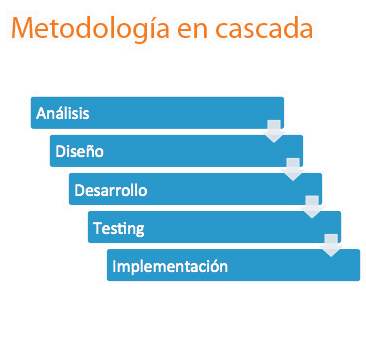
\includegraphics[width=0.6\textwidth]{imagenes/03_Planificacion/meto_clasica.jpg}
    \caption{Etapas de la metodología clásica (Fuente: https://www.yunbitsoftware.com/blog/2016/05/20/desarrolo-de-software-metodologias-waterfall-agile)}
    \label{fig:etapas_clasica}
\end{figure}

Dado que la metodología clásica sólo consta de un ciclo para realizar las etapas, será imprescindible una buena planificación de alcance, tiempo y coste del proyecto y de cada una de las etapas. Esta planificación inicial es tan importante porque no se obtendrán resultados del proyecto hasta que se encuentre cercano a su cierre.

Entre los problemas de la metodología clásica podemos encontrar los siguientes:

\begin{itemize}
    \item Los proyectos reales difícilmente se adecuan a este modelo de proceso.
    \item Dificultad para expresar por parte del cliente todos los requisitos al principio del proyecto.
    \item Poca comunicación con cliente/usuario, hasta las etapas finales no hay un ejecutable que se pueda evaluar.
\end{itemize}


\subsubsection{Metodología Ágil}

Esta metodología surge como solución a los problemas de la metodología clásica, sobretodo para la planificación de proyectos cortos y cambiantes. La metodología ágil se caracteriza por su flexibilidad, durante el desarrollo del proyecto la planificación sufre continuos cambios debido a la constante comunicación con el usuario; una estructura incremental, con esta metodología no se obtiene un único proyecto final, si no más bien se van generando prototipos que se van analizando y mejorando en un retroalimentación constante, aumentando la colaboración; y un flujo de proceso iterativo, a diferencia de la metodología clásica donde cada etapa una vez finalizada no se vuelve a ella teniendo un flujo en cascada, en esta metodología el flujo de las etapas es más parecido a un círculo convertido en un bucle sin fin. Esta metodología se adapta mejor a los proyectos del ámbito de las TIC, es decir, en el desarrollo de software, donde es fundamental la flexibilidad del proyecto y el carácter incremental de la metodología. Este modo de trabajar no se adecua a proyecto que puedan estar relacionados con sectores alejados de las TIC como puede ser el sector de la construcción, por ejemplo en la construcción de un puente, dado que no se pueden crear prototipos de una construcción ya que no serían seguros, y además son proyectos poco cambiantes en los requisitos del proyecto durante su desarrollo.

El ciclo de etapas de la metodología ágil se puede visualizar en la Figura \ref{fig:etapas_agil}.

\begin{figure}[h]
    \centering
    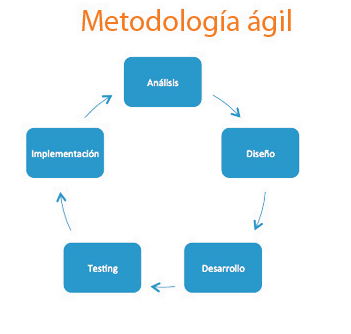
\includegraphics[width=0.6\textwidth]{imagenes/03_Planificacion/meto_agil.jpg}
    \caption{Etapas de la metodología ágil (Fuente: https://www.yunbitsoftware.com/blog/2016/05/20/desarrolo-de-software-metodologias-waterfall-agile)}
    \label{fig:etapas_agil}
\end{figure}

Dentro de la categoría de metodología ágil podemos encontrar las siguientes metodologías:

\begin{itemize}
    \item Scrum
    \item Programación exterma (XP)
    \item Mobile-D
\end{itemize}

En mi caso me voy a centrar en la metodología Scrum, muy popular hoy en día en la planificación de proyectos TIC. Tal y como se indica en el artículo (Referencia a Articulo metodología), Scrum no corresponde a ningún acrónimo, su nombre proviene del deporte rugby, que es una formación requerida para la recuperación rápida del juego ante una infracción menor. Esta metodología se caracteriza por el empleo de un conjunto de reglas y la definición de roles. La existencia de estos roles favorece una colaboración eficaz del equipo de trabajo. 
Los roles que se definen son: El Scrum master, el dueño del producto o Product owner y el equipo de desarrollo o team. El scrum master es la persona que lidera el equipo asegurándose que el equipo cumpla las reglas y procesos de la metodología. El dueño del producto es el representante de los accionistas y clientes que usan el software. El equipo de desarrollo es el grupo de profesionales encargados de convertir la lista de requerimientos o también llamado Product Backlog en funcionalidades del software (Referencia a Articulo metodología).

La característica incremental de las metodologías ágiles se materializa en la metodología Scrum como un elemento llamado Sprint (Figura \ref{fig:sprint_scrum}). Cada sprint consistirá en un recorrido completo de todas las etapas del proyecto, dando como resultado una versión utilizable del producto.

Los elementos de un sprint son los siguientes:

\begin{itemize}
    \item Reunión de planificación del sprint
    \item Daily Scrum ó reunión diaria
    \item Trabajo de desarrollo
    \item Revisión
    \item Retrospectiva del sprint
\end{itemize}

Durante la reunión de planificación del sprint se seleccionan que tareas se van a desarrollar en ese sprint. Las tareas son extraídas del Product Backlog, que no es más que una lista de tareas ordenas por prioridad. Esta lista será actualizada y modificada durante el desarrollo del proyecto.

\begin{figure}[h]
    \centering
    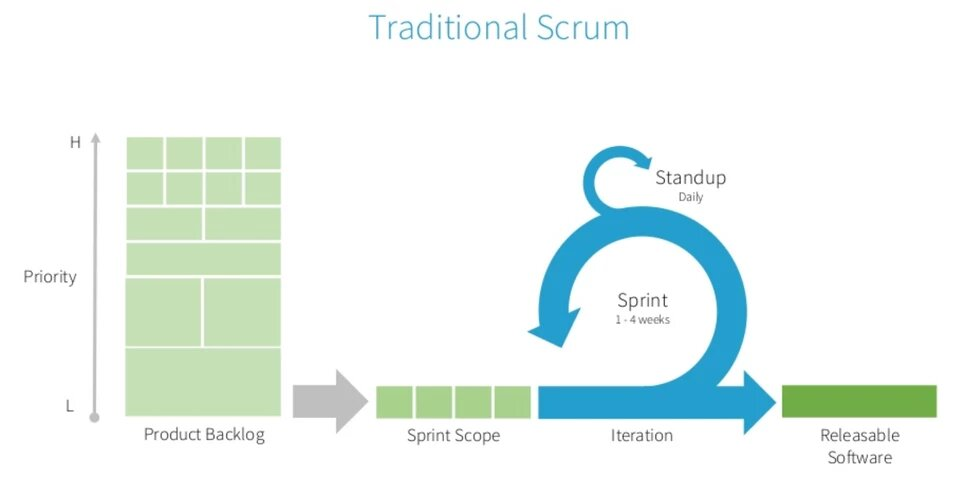
\includegraphics[width=0.8\textwidth]{imagenes/03_Planificacion/sprint_scrum.jpg}
    \caption{Sprint de la metodología Scrum (Fuente: https://openwebinars.net/blog/que-es-un-sprint-scrum)}
    \label{fig:sprint_scrum}
\end{figure}


\subsection{Aplicación de Scrum al proyecto}

Tomando como partida la metodología Scrum original, se ha realizado una adaptación a mi proyecto. La primera adaptación es la asignación de roles, donde una misma persona realiza los tres roles a la vez, dado que el equipo de desarrollo del proyecto lo forma una única persona; y como añadido el papel de usuario lo realizará el tutor del proyecto. Otra consecuencia, derivada de la formación del equipo por una única persona, es que no van a realizar reuniones diarias dado que no hay que realizar una supervisión del trabajo del equipo en conjunto. Aunque no se realicen reuniones diarias se ha optado por realizar autorreflexiones semanalmente para llevar un control del avance durante el sprint. Los sprints tendrán una duración inicial de 4 semanas. Además de las propias autorreflexiones, se realizarán reuniones con el tutor cada dos semanas, es decir, inicialmente estas reuniones se producirán a mitad de cada sprint y al final del mismo, aunque el contacto con el tutor es constante durante todo el sprint.

Además de aplicar la metodología Scrum, he optado por aplicar la metodología DevOps. Esta metodología busca la transparencia entre el equipo que desarrolla el software y el equipo que se encarga del despliegue del mismo.




\chapter{Análisis}


\section{Tecnologías de desarrollo}

Un aspecto a tener en cuenta a la hora de elegir una plataforma para desarrollar un chatbot es que existen dos elementos en esta creación.

\begin{itemize}
    \item \textbf{Bot Frameworks}: son las plataformas encargadas de la creación y el alojamiento de los chatbots.
    \item \textbf{Bot Platforms}: son los entornos y aplicaciones donde van a ser desplegados los chatbots para su uso por parte de los usuarios.
\end{itemize}

A la hora de elegir la plataforma donde desarrollar el chatbot habrá que tener en cuenta que tanto el Bot Framework como el Bot Platform elegidos se adecuan a los requisitos del chatbot a crear.

Una posible clasificación de las plataformas puede ser en base al modo de creación de los chatbots. Dentro de esta clasificación encontramos las siguientes plataformas:

\begin{itemize}
    \item \textbf{Plataformas visuales}
    \item \textbf{Plataformas conversacionales}
    \item \textbf{Plataformas programables}
\end{itemize}

\subsubsection*{Plataformas visuales}

En estas plataformas no es necesario tener conocimientos técnicos para crear un chatbot. Por esta razón son las plataformas ideales para personas que no tienen conocimientos en programación ó IA. Algunos ejemplos de este tipo de plataformas pueden ser: Chatfuel y Octane AI. Esta simpleza en la creación del chatbot afecta en la posible complejidad que pueda tener el chatbot, por lo tanto no son las mejor opción para chatbots con con algo de complejidad, pero si para chatbots muy simples.

\subsubsection*{Plataformas conversacionales}

En estas plataforma es posible la creación de chatbots algo más complejos que en las plataformas visuales. Estos chatbots son capaces de mantener una conversación con un usuario, pero que a diferencia de los anteriores chatbots esta conversación no tiene un objetivo específico. Un posible ejemplo de este tipo de plataformas puede ser AIML, aunque AIML no es en sí una plataforma sino más bien un lenguaje de programación, si se convierte en una plataforma si se combina el lenguaje con alguna plataforma donde se permita al menos el alojamiento del chatbot. Este tipo de plataformas ya no está orientado a usuarios sin conocimientos técnicos, sino más bien a usuarios que tengan cierto nivel técnico y que busquen crear chatbots con cierta complejidad. 

\subsubsection*{Plataformas programables}

En estas plataforma se pueden crear desde los chatbots más simples hasta los más complejos. Para poder aumentar la complejidad se hace uso de técnicas de IA junto a las técnicas que ya se utilizaban en las anteriores plataformas, y aumenta la posibilidad de interactuar con servicios externos a la plataforma como pueden ser bases de datos y muchos más servicios. Algunos ejemplos de este tipo de plataformas pueden ser: Google Dialogflow, Microsoft Bot Framework y IBM Watson. \newline\newline


En la actualidad se dispone de un número elevado de plataformas capaces de crear chatbots de diferentes complejidades. De entre este número elevado de plataforma he seleccionado unas cuantas para analizarlas en detalle como posibles plataformas donde crear mi chatbot. En esta lista de plataformas no se encuentra ninguna plataforma visual dado que no posibilitan la complejidad necesaria para crear mi chatbot.


\subsection{AIML}

\subsubsection*{Información general}

El lenguaje de programación AIML (Artificial Intelligence Markup Language) fue desarrollado por el doctor Richard Wallace y la comunidad de código abierto Alicebot en la segunda mitad de los años 90. AIML es un lenguaje basado en etiquetas, al igual que los lenguajes HTML y XML. En concreto el lenguaje AIML se baso en gran medida en el lenguaje XML. Este parecido entre lenguajes no es una casualidad, si nos fijamos en el entorno de la época en la que se desarrollo AIML. A finales de la década de 1990 se produjo la explosión de la World Wide Web. Esta explosión trajo consigo al lenguaje HTML, que surgió como un lenguaje simple que sirviese como estándar para la creación de páginas web. El objetivo de HTML era que cualquier persona con pocos conocimientos informáticos fuese capaz de crear una página web. Esta filosofía de estándar de una tecnología y de simpleza la tomaron como ejemplo los creadores de AIML durante su desarrollo, intentando que AIML se convirtiese en un estándar en la creación de chatbots y que además fuese accesible al mayor número de usuarios. Además del lenguaje HTML, durante la década de 1990 se creo el lenguaje XML, que también se convirtió en un estándar.

Actualmente, al igual que le ha pasado al lenguaje HTML, el lenguaje AIML se ha ido actualizando con el tiempo añadiendo le nuevas funcionalidades que permitiesen crear chatbots más complejos, acorde al incremento de requisitos en los chatbots que ha ido surgiendo con el paso de los años. En el momento de la realización de este TFG, la última versión publicada de AIML es la versión 2.1 . Al crear agentes conversacionales con AIML, estos agentes no se convierten en cajas negras por lo tanto son más transparentes al programador que los creados con otras plataformas más grandes, ya que con AIML se crean chatbots basados en reglas. AIML se puede escribir en casi cualquier lenguaje natural.



→ http://www.aiml.foundation

\subsubsection*{Uso}

Para crear un chatbot con AIML es necesario generar una serie de archivos, que contendrán el estado y la configuración del bot.

En el estado del chatbot podemos distinguir el estado del bot y el estado del cliente. El estado del bot se define usando valores globales para las propiedades del bot, cada bot tendrá sus propiedades. El estado del cliente se define usando variables locales, cada cliente tendrá su estado específico.

La configuración del bot se define en los archivos AIML, en los archivos Learnf, en los Sets y en los Maps. Dentro de los archivos AIML se define la lógica del chatbot a base de añadir reglas, además en estos archivos se pueden realizar conexiones con otros chatbots definidos por otra serie de archivos. Dentro de los archivos Learnf se guardan las categorías aprendidas por el chatbot cuando en un template AIML se activa una etiqueta. Las categorías parendidas son globales a todos los clientes del chatbot. Dentro de los archivos Set se define un conjunto de cadenas. Dentro de los archivos Map se define un mapeo de cadena a cadena.

Según el estándar de AIML, esta serie de archivos se pueden definir dónde y cómo quiera el creador del chatbot.

Dado que AIML es sólo un lenguaje de programación, es necesario un framework para la creación del agente conversacional, como pueden ser algunos intérpretes y bibliotecas de código abierto (Python, Node JS, Java) ó servicios web (Pandorabots).

Si se elige la opción de usar intérpretes y bibliotecas de código abierto disponemos de las siguientes posibilidades:

\begin{itemize}
    \item Python $\rightarrow$ Program-Y
    \item Node JS $\rightarrow$ aimlinterpreter
    \item Java $\rightarrow$ Program AB
\end{itemize}

Si se elige la opción de usar servicios web como Pandorabots, uno de los más populares actualmente, se podrá alojar el chatbot en la plataforma y se podrá hacer uso de todas sus funcionalidades. Si nos centramos en Pandorabots disponemos de un editor de AIML, un editor de interfaces, control de versiones a través de Github, chatlogs, conversor de texto a voz y viceversa, posiblidad de añadir un personaje 3D como interación con el chatbot, integración con RESTful APIs y muchos más, según se indica en su página oficial \cite{RefWorks:RefID:14-pandorabots:}.

Muchas de estas funcionalidades depende del tipo de cuenta que se disponga en Pandorabots.

\newpage

\begin{figure}[h]
    \centering
    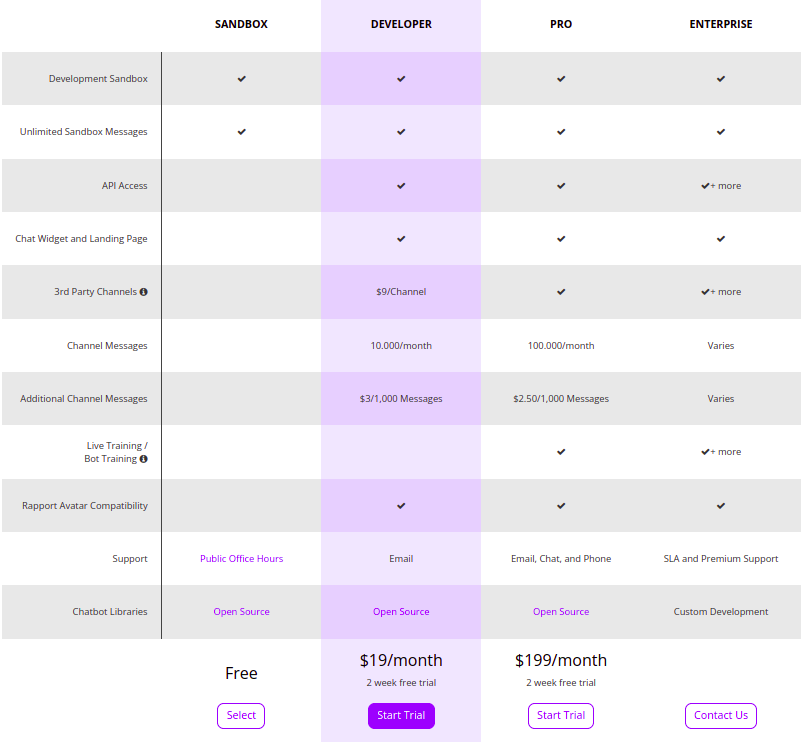
\includegraphics[width=1.0\textwidth]{imagenes/04_Analisis/cuentas_pandorabots.png}
    \begin{center}
        Fuente: \url{https://developer.pandorabots.com/home.html}
    \end{center}
    \caption{Cuentas disponibles en Pandorabots}
    \label{fig:cuenta_pandorabots}
\end{figure}

En la figura \ref{fig:cuenta_pandorabots} podemos comprobar como con la cuenta gratuita no disponemos de todas las funcionalidad anteriormente descritas.


→ https://developer.pandorabots.com/


\subsubsection*{Extensibilidad}

Dado que hay muchos frameworks para la creación de un chatbot con AIML, dependerá del framework elegido la cantidad de posiblidades de conexiones con APIs o servicios externos al chatbot. 

Para que AIML sea flexible y extensible dispone de la posibilidad de integrar sus propias API's, bases de datos ó también se pueden crear etiquetas propias; pero para ello se debe tener cierto nivel con el lenguaje de programación AIML.

Si optamos por servicios web como Pandorabots para poder disponer de conexión con servicios externos al servicio web o con APIs se debe disponer de una cuenta de pago, no basta con la versión gratuita de Pandorabots.

\subsubsection*{Integración}

Si optamos por servicios web como Pandorabots, al igual que pasa con la extensibilidad, será necesaria una cuenta de pago para poder integrar nuestro chatbot en plataformas de mensajería como Facebook Messenger, Twitter, Telegram y muchos más.

Pero si optamos por framework de código abierto hay una multitud de posibilidades, tantas como nivel de conocimientos tenga el creador del chatbot. Un ejemplo puede ser con Node JS, donde podríamos desplegar el chatbot en cualquier página web a través de una interfaz web que enviase peticiones al servidor creado con Node JS que aloja al chatbot.

\subsubsection*{Ejemplos}

Algunos ejemplos de chatbot implementados con AIML son los siguientes:

\begin{itemize}
    \item \textbf{Rosie}. Chatbot base basado en ALICE 2.0 \footnote{\url{https://github.com/pandorabots/rosie}}
    \item \textbf{Programa-Y}. Chatbot basaso en Python 3.x y AIML 2.0 \footnote{\url{https://github.com/keiffster/program-y}}
    \item \textbf{Cathy}. Chatbot para Discord basado en Python 3 y AIML \footnote{\url{https://github.com/DevDungeon/Cathy}}
\end{itemize}


\subsection{IBM Watson}

\subsubsection*{Información general}

IBM Watson es un portfolio de IBM de aplicaciones, herramientas y soluciones preparadas para la empresa, diseñado para reducir los costes y los obstáculos de IA, además de optimizar los resultados y el uso responsable de la IA según se indica en su página oficial \cite{RefWorks:RefID:15-2021ibm}. Aunque en un inicio IBM Watson no era lo que es ahora actualmente y tampoco se buscaba llegar a este punto. Originalmente IBM Watson surgío como el siguiente gran desafío de la empresa IBM, tras haber salido victorioso de otros grandes desafíos como la victoria de Deep Blue contra Garry Kasparov y el desafío de la supercomputadora Blue Gene. El objetivo que perseguía en sus orígenes Watson era conseguir ganar a competidores humanos en el concurso Jeopardy. Este concurso de televisión estadounidense consistía en un concurso de preguntas sobro una multitud de temas, y los concursantes deberán resolver las preguntas de cada prueba realizando preguntas sobre las pistas que va dando el presentador. Las reglas del concurso obligan a que Watson no sólo sepa conocimientos sobre los temas que se utilizan en el concurso, sino también ha saber realizar preguntas al presentador en base a sus pistas, y además saber distinguir cuando la pista del presentador no es cierta. Todas estos requisitos convierten el ganar este concurso en un gran desafío, la empresa IBM se embarco en este proyecto a mediados de la década del 2000. Finalmente en el año 2011 se llegó a un acuerdo para la realización del programa, donde compitieron dos grandes exconcursantes del programa como son Ken Jennings y Brad Rutter contra Watson. Tal y como se indica en el articulo \cite{RefWorks:RefID:16-best2013ibm}, Watson ganó el juego con \$77,147 , dejando a Rutter y Jennings con \$21,600 y \$24,000 respectivamente.

Tras la victoria de IBM Watson, se empezó a enfocar y rediseñar a Watson hacia distintos sectores como la medicina, la banca ó los agentes conversacionales entre otras. Los agentes conversacionales es el sector que nos interesa investigar.

Dado que IBM Watson está orientado al mundo empresarial destaca por su confianza, es decir, Watson es transparente en cuanto a las decisiones basadas en IA; también protege la privacidad de los datos y su seguridad. Todas estas características son muy valoradas en cualquier producto empresarial, incluso algunas son imprescindibles.

Otro característica de Watson es su procesamiento del lenguaje natural. Al igual que AIML es multilenguaje, pero Watson lo lleva a un aspecto más complejo añadiendo la capacidad de analizar datos complejos y no estructurados, como pueden ser códigos de programación ó incluso formas de expresión específicas de una modalidad de trabajo. Este procesamiento del lenguaje natural no es algo alcanzable por cualquier empresa. La IA de Watson sabe desenvolverse en la situaciones más complejas, como pueden ser situaciones en las que no pueda responder, reenviando la solicitud a un agente humano o hacia algún documento de ayuda; evitando realizar preguntas redundante facilitando la comunicación y haciéndola más natural; y por última sabe manejar solicitudes ambiguas comunes en la comunicación como pueden ser errores ortográficos, cambios de tema, y muchas más situaciones que pueden ser inesperadas para el chatbot en una conversación. Además IBM Watson intenta mejorar su rendimiento aportando al creador del chatbot información sobre que nuevos temas añadir para mejorar la respuesta a las solicitudes.

Y por último destaca que Watson trabaja con cualquier servicio en la nube, lo que facilita su integración en las empresas, ya que no será un impedimento el lugar donde residan los datos de la empresa. Y además el trabajar en cloud facilitará el trabajo con los datos.

En concreto en la página oficial de IBM Watson Assistant \cite{RefWorks:RefID:17-ibm} se destaca la rentabilidad del producto, de hasta un 337\% según el Informe TEI de Forrester \cite{RefWorks:RefID:8-iles2020el}; su precisión, de hasta un 14,7\% superior que las soluciones de la competencia según un reciente estudio publicado sobre machine learning \cite{RefWorks:RefID:18-2020watson}; y su fiabilidad, ya que Watson tiene más de 1000 despliegues de clientes en todos los sectores.



→ https://www.ibm.com/es-es/watson

→ El Total Economic Impact™ de IBM Watson Assistant

→ https://www.ibm.com/es-es/products/watson-assistant

→ https://www.techrepublic.com/article/ibm-watson-the-inside-story-of-how-the-jeopardy-winning-supercomputer-was-born-and-what-it-wants-to-do-next/

→ https://www.ibm.com/blogs/watson/2020/12/watson-assistant-improves-intent-detection-accuracy-leads-against-ai-vendors-cited-in-published-study/

\subsubsection*{Uso}

IBM Watson está pensado para ser utilizado por cualquier persona, da igual que no tenga conocimientos en programación. La creación del chatbot se basa en un editor de arrastrar y soltar. Este editor evita la complejidad de la programación de un chatbot y los posibles errores derivados de esa necesidad de escribir el código en su creación ó en alguna modificación que necesite el chatbot. Es posible crear un chatbot sin escribir una sola línea de código.

\begin{figure}[h]
    \centering
    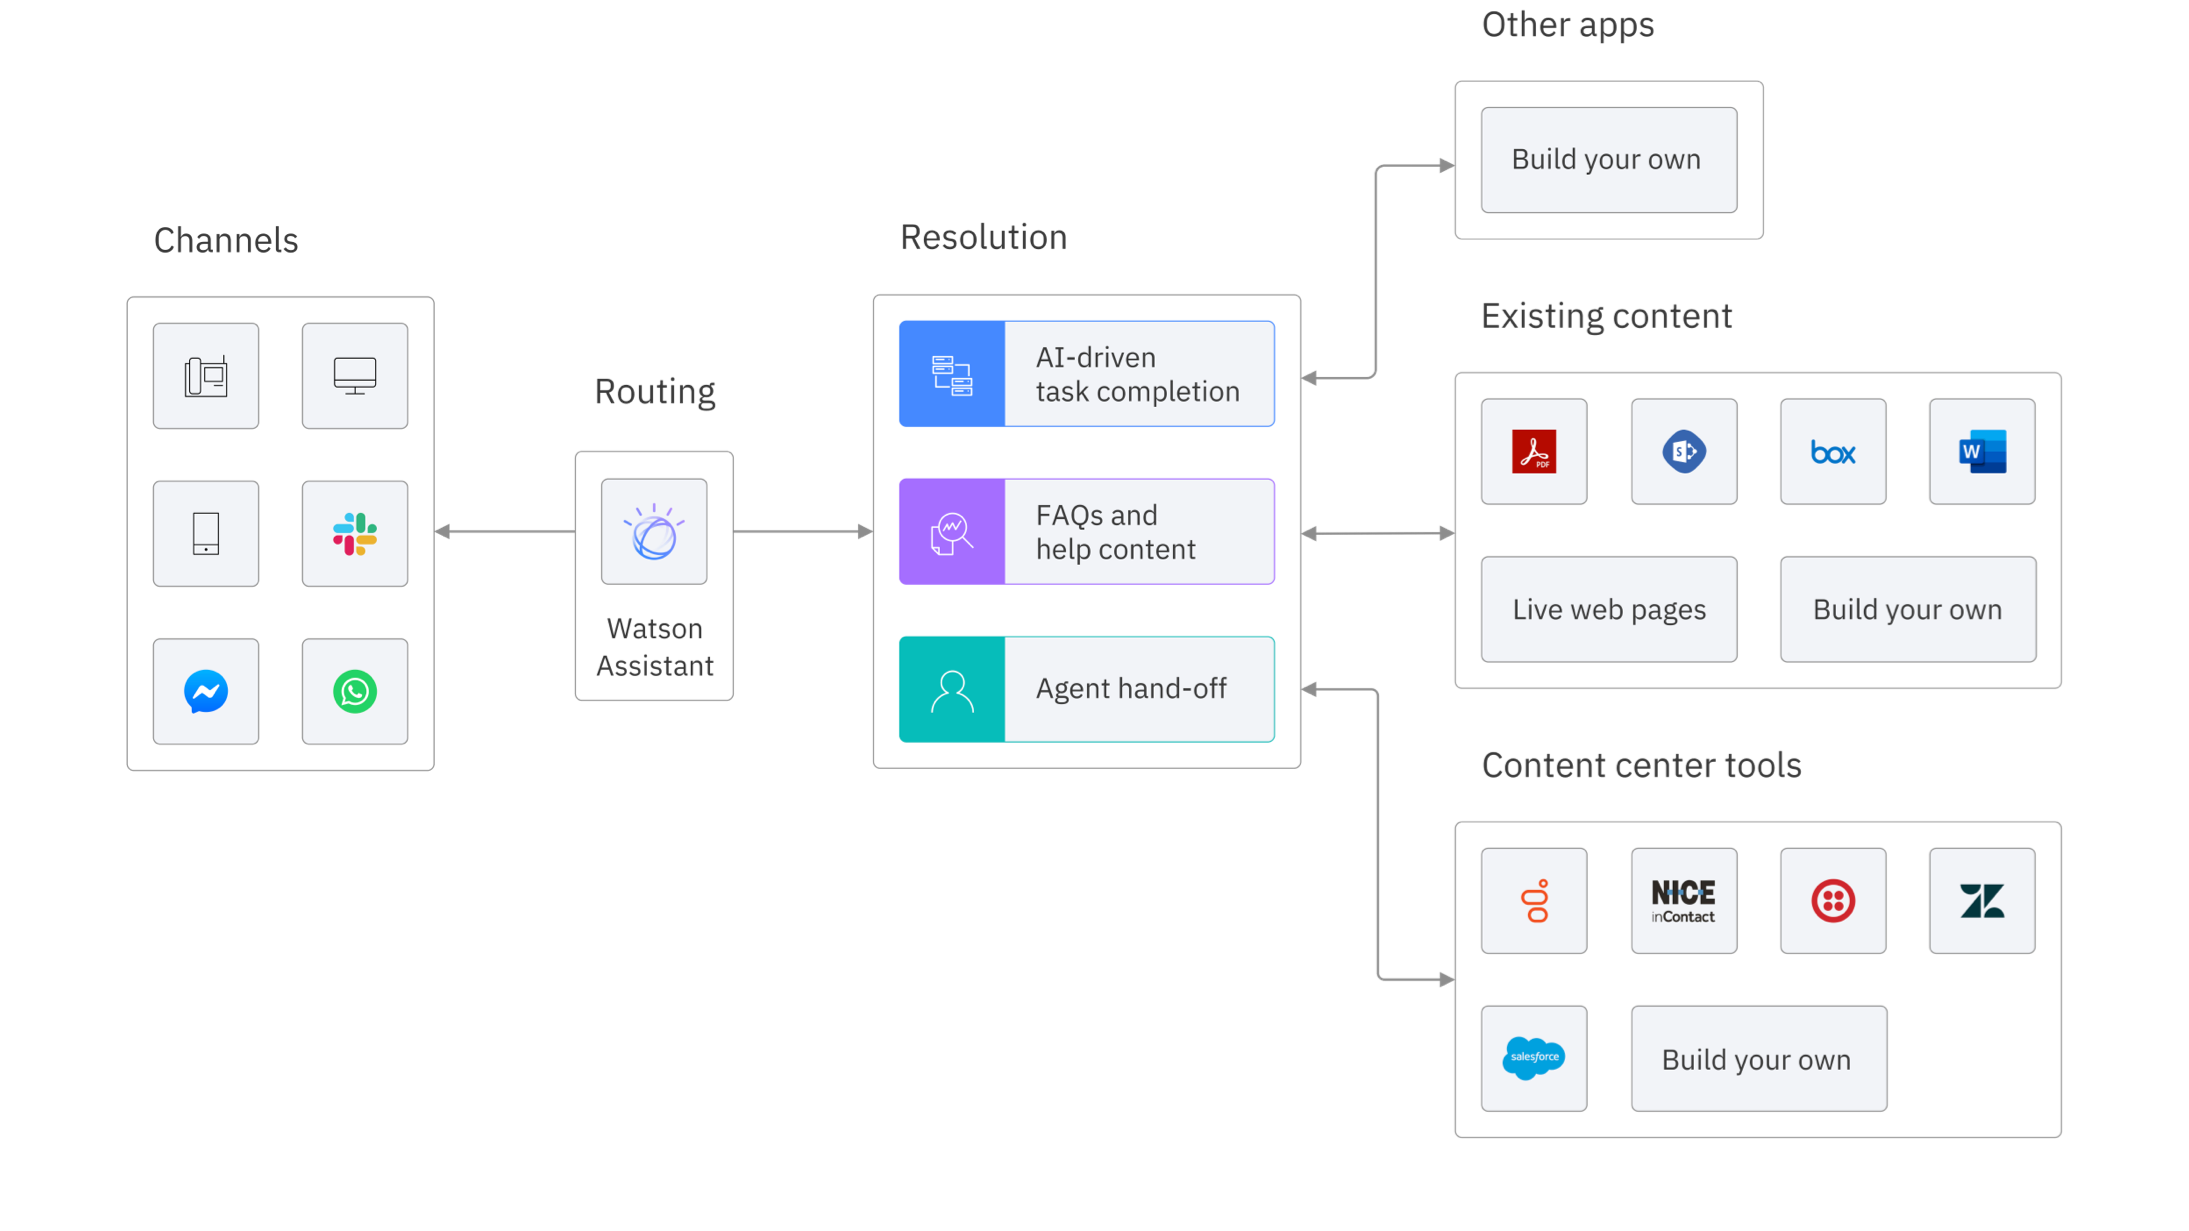
\includegraphics[width=1.0\textwidth]{imagenes/04_Analisis/editor_IBM_Watson.png}
    \begin{center}
        Fuente: \url{https://www.ibm.com/es-es/products/watson-assistant}
    \end{center}
    \caption{Editor de IBM Watson}
\end{figure}

La IA del chatbot es capaz de comprender un tema en cualquier lenguaje natural con unas pocas frases facilitando la adaptación del chatbot a la funcionalidad que se le quiera dar, adaptándose de forma rápida y precisa al dominio del proyecto.

\subsubsection*{Extensibilidad}

Como se ha indicado en apartados anteriores, IBM Watson es un portfolio de IBM de aplicaciones. En su página oficial \cite{RefWorks:RefID:19-2021productos} se indican las siguientes aplicaciones con las que se puede integrar el chatbot:

\begin{itemize}
    \item IBM Watson Discovery
    \item IBM Watson Natural Language Understanding
    \item IBM Watson Speech to Text
    \item IBM Watson Text to Speech
    \item IBM Watson Knowledge Studio
    \item IBM Watson Language Translator
    \item IBM Watson Natural Language Classifier
\end{itemize}

Entre estas aplicaciones se encuentran algunas muy útiles como IBM Watson Discovery para la extracción y búsqueda de información, IBM Watson Speech to Text para transformar la voz a texto escrito gracias a una potente tecnología de machine learning, IBM Watson Language Translator para traducir dinámicamente información, ó IBM Watson Knowledge Studio para enseñar a Watson el idioma del domino del chatbot.



→ https://www.ibm.com/es-es/watson/products-services

\subsubsection*{Integración}

El chatbot se puede integrar como un chat web, como contestador de llamadas de teléfono ó como un chatbot en una aplicación de mensajería como WhatsApp, Facebook Messenger, SMS y muchos más. Todas estas formas de integrar el chatbot son muy fáciles de realizar.

\subsubsection*{Ejemplos}

Algunos ejemplos de chatbot implementados con Watson son los siguientes:

\begin{itemize}
    \item \textbf{Nanci. Chatbot desarrollado por la empresa GM Financial} \footnote{\url{https://www.gmfinancial.com/en-us/company/newsroom/chatbot.html}}
    \item \textbf{Chatbot desarrollado por la empresa Bradesco} \footnote{\url{https://www.ibm.com/watson/stories/bradesco}}
    \item \textbf{CARL. Chatbot desarrollado por la empresa Siemens} \footnote{\url{https://www.ibm.com/es-es/products/watson-assistant/client-stories}}
    \item \textbf{Chatbot desarrollado por la empresa Humana} \footnote{\url{https://www.ibm.com/watson/stories/humana}}
\end{itemize}




→ https://www.ibm.com/watson/stories/humana
→ https://www.ibm.com/es-es/products/watson-assistant/client-stories
→ https://www.ibm.com/watson/stories/bradesco
→ https://www.gmfinancial.com/en-us/company/newsroom/chatbot.html


\subsection{Google Dialogflow}\label{subsec:dialogflow}

\subsubsection*{Información general}

Dialogflow pertenece a la empresa Google, aunque no fue desarrollada originalmente por ella. Google adquirió API.AI en el año 2016 y le cambió el nombre a Dialogflow. Desde su adquisición Google a mejorado Dialogflow gracias a sus técnicas de IA de gran calidad. Esta plataforma es una de las más utilizadas para la creación de chatbots junto con IBM Watson, aunque a diferencia de Watson, Dialogflow está enfocado tanto para el mundo empresarial como para usuarios particulares que están empezando en el mundo de los chatbots. Esta variedad en la complejidad del chatbot es posible gracias a una interfaz que permite crear un chatbot con unos mínimos conocimientos técnicos, sólo será necesario introducir las frases de las preguntas y de las respuestas para construir el chatbot. Y si se quiere crear un chatbot más complejo podemos introducirnos en la configuración del chatbot o integrar más funcionalidades que aumenten su complejidad.

Dentro de Dialogflow existen dos tipos de agentes, los Agentes de ES y los agentes de CX. Dentro de los agentes de ES existen dos ediciones, la edición de prueba y la edición Essentials. Con la versión de prueba no se puede acceder a los servicios de Google Cloud, pero las entradas y salidas son gratuitas; mientras que con la versión Essentials si se puede acceder a esos servicios, pero las entrada y salidas del agente empezarán a costar dinero. Entre la versión Essentials y la versión CX la principal diferencia es que en la versión CX la relación entre los intents se define mediante un diagrama de flujo, mientras que en la versión Essential la relación entre los intents se define mediante los contextos. La limitación de los contextos es que no posibilitan la relación de varios intents con otro intent. La versión CX ha sido lanzada hace pocos unos pocos meses por lo que es algo novedosa y es útil para aquellos que quieran realizar un chatbot algo más complejo o que ya tengan experiencia con la plataforma. La versión Essentials está más enfocada a agentes de complejidad media y la versión CX está más enfocada a agentes de complejidad alta. Aunque la curva de aprendizaje es más suave en la edición CX, la edición CX no dispone actualmente de todas las funcionalidades presentes en la edición Essentials.

\subsubsection*{Uso}

Para empezar a crear un chatbot con Dialogflow será necesaria una cuenta Google. Los apartados claves para la creación de un bot son Intents y Entities.

Dentro del apartado Intents se crean los distintos intents a usar en el chatbot, cada intent es un estado al que accede el chatbot si se cumple el contexto y se detecta una de las frases de entrenamiento del intent. Los contextos sirven para guardar información adquirida que puede resultar útil durante la conversación, como el nombre del usuario que está usando el chatbot; además de la información que se quiere conservar también se puede indicar durante cuento tiempo se estima que es útil esa información, también llamado lifespan. Dentro de cada intent se debe también definir las posibles respuestas que envía el chatbot si se activa el intent. Y por último a cada intent se le pueden añadir eventos. Por defecto en el apartado Intents vienen creados los siguientes intents:

\begin{itemize}
    \item Default Fallback Intent: Intent para cuándo el chatbot no reconoce la pregunta
    \item Default Welcome Intent: Intent para dar la bienvenida al chatbot
\end{itemize}

Dentro del apartado Entities se crean las distintas entidades. Una entidad es un conjunto de ejemplos sobre un tema, por ejemplo la entiedad paises contiene los siguientes elementos: España, Francia, Italia, etc. Cuando se define una entidad se deben indicar los elementos que la forman, pero adicionalmente se puede indicar los sinónimos de los elementos, este añadido le dará una mayor naturalidad a la conversación al hacer que los textos no sean tan estáticos.

Otro apartado importante para el desarrollo del chatbot es el apartado Training, donde se podrán analizar las conversaciones que se han realizado con el chatbot e indicar si se ha respondido adecuadamente o no, esta acción de aceptación o no hará que el chatbot sea más preciso con sus respuestas. Si se acepta una respuesta, si la pregunta realizada por el usuario no se encuentra entre las preguntas del intent activado, se añade a la lista de preguntas del intent.

\subsubsection*{Extensibilidad}

Dialogflow permite integrar un webhook. Este webhook puede estar alojado tanto en un servidor externo como en Google Cloud. Si se opta por la opción de Google Cloud, para lo que es necesario una cuenta Google de pago, se pueden añadir los archivos que componen el webhook en el apartado Fulfillment dentro de un editor en linea. Si se opta por la opción de un servidor externo, tanto si es local como si es en una plataforma en la nuebe, se deberá añadir la URL del servidor web en el mismo apartado que se indicó anteriormente. La conexión con el servidor externo se realizará mediante el envío de peticiones tipo POST. Estas peticiones contendrán la información en formato JSON. Para que la información se envíe al servidor, independientemente de la opción que se elija, se debe activar en los intents elegidos la opción del webhook, de esta forma cuando se active el intent se enviará una petición al servidor web.

Una vez se tenga una conexión con un servidor web, dentro de este servidor se podrán añadir más funcionalidad, como BBDD ó interpretes de AIML, que permitirán seguir extendiendo el chatbot.

\subsubsection*{Integración}

El chatbot se puede integrar en canales de telefonía, como Twilio; en canales de mensajería, como Telegram, Facebook Messenger ó Twitter; en canales de videollamadas, como Skype; y en páginas web en forma de chat web.

\subsubsection*{Ejemplos}

Algunos ejemplos de chatbot implementados con Dialogflow son los siguientes:

\begin{itemize}
    \item \textbf{SAM. Chatbot desarrollado por la empresa Ubisoft} \footnote{\url{https://www.hd-tecnologia.com/ubisoft-ia-personal-sam-primer-asistente-gaming}}
    \item \textbf{Chatbot desarrollado por la empresa Dominos Pizza} \footnote{Caso de estudio de Dominos Pizza \cite{RefWorks:RefID:10-domino's-case-study}}
    \item \textbf{Chatbot desarrollado por la empresa Malaysia Airlines} \footnote{\url{https://cloud.google.com/customers/malaysia-airlines}}
\end{itemize}


→ https://www.hd-tecnologia.com/ubisoft-ia-personal-sam-primer-asistente-gaming
→ https://cloud.google.com/customers/malaysia-airlines


\subsection{Rasa Stack}

\subsubsection*{Información general}

Rasa Stack es un conjunto de herramientas de aprendizaje automático de código abierto para el desarrollo de chatbots. Rasa Stack está desarrollado por una comunidad de personas pertenecientes a muchos lugares del mundo, de modo que esta plataforma a diferencia de las dos anteriores, no está respaldado por ninguna de las grandes empresas tecnológicas como pueden ser Google o IBM. Pero esto no quiere decir que no sea una buena plataforma, ya que ha sido probada por grandes empresas como AIRBUS, TOYOTA ó Adobe.

En su página oficial \cite{RefWorks:RefID:20-2020rasa} se destaca la gran personalización que pueden alcanzar los chatbots en esta plataforma.

Dentro de Rasa Stack se pueden distinguir dos tipos de cuenta, la cuenta para empresas (Rasa Enterprise) y la cuenta gratuita (Rasa Open Source ó Rasa X). La diferencia entre Rasa Open Source y Rasa X es que Rasa X no es de código abierto, mientras que Rasa Open Source, como indica su nombre, si es de código abierto. La cuenta para empresas proporciona funcionalidades muy útiles para productos empresariales como pueden ser realizar análisis del chatbot, acceso con roles a la plataforma, disponibilidad de un soporte de calidad, y mucho más.

En Rasa Stack se destaca que los chatbot creados en esta plataforma no se convierten en cajas negras, sino que el funcionamiento del chatbot es transparente, por lo tanto se tiene total acceso a la configuración de todo el chatbot, incluido el modelo usado en el entrenamiento del bot.


→ https://rasa.com

\subsubsection*{Uso}

Al igual que pasa en Dialogflow, Rasa Stack mantiene un contexto de la conversación, donde se guarda información proporcionada por el usuario, lo que permite una conversación más natural al no realizar preguntas redundantes.

La creación del chatbot se divide en dos módulos, Rasa NLU y Rasa Core. La plataforma proporciona un NLU avanzado, Rasa NLU, esta NLU se puede entrenar en base a una lista de mensajes, a cada mensaje se le asignará una intención y las entidades que contiene. Una vez está entrenado el módulo NLU, se procede a configurar el módulo Rasa Core, que es el encargado de confeccionar la respuesta del chatbot a la pregunta identificada por el módulo Rasa NLU. La configuración de Rasa Core consiste en escribir las respuestas de los distintos intents, definir el dominio del chatbot, definir la conexiones con APIs, y definir el modelo de gestión del diálogo, por ejemplo una CNN, citando además las políticas que se van a usar.

\subsubsection*{Extensibilidad}

La transparencia que tienen los chatbots permiten conectar con él muchas APIs externas que suman más funcionalidades a parte de las que ya proporciona la plataforma. Y al igual que pasa con Dialogflow, se puede conectar a un servidor web y al servidor las APIs.

\subsubsection*{Integración}

Tal y como se indica en su página oficial \cite{RefWorks:RefID:20-2020rasa}, un chatbot creado con Rasa Stack se puede integrar en canales como IVR, chat y SMS. Además se indica que Rasa Stack admite 10 canales de mensajería integrados, como pueden ser Telegram, Facebook Messenger, Slack y algunos más; y que adicionalmente proporciona un punto de conexión con cualquier plataforma de comunicación, como puede ser un servidor web.

\subsubsection*{Ejemplos}

Algunos ejemplos de chatbot implementados con Rasa Stack son los siguientes:

\begin{itemize}
    \item \textbf{Djingo. Chatbot desarrollado por la empresa Orange} \footnote{\url{https://rasa.com/customers/orange}}
    \item \textbf{Chatbot desarrollado por la empresa TMobile} \footnote{\url{https://rasa.com/customers/t-mobile}}
    \item \textbf{Chatbot desarrollado por la empresa Helvetia} \footnote{\url{https://rasa.com/customers/helvetia}}
\end{itemize}



→ https://rasa.com/customers/helvetia
→ https://rasa.com/customers/orange
→ https://rasa.com/customers/t-mobile


\subsection{GPT-3}

\subsubsection*{Información general}

GPT-3 (Generative Pre-trained Transformer 3) es un conjunto de modelos de inteligencia artificial desarrollado por la empresa OpenAI en el año 2020. Este modelo es la tercera generación de estos modelos de inteligencia artificial. Este último modelo tiene 175 billones de parámetros, lo cuál es una potencia impresionante que le permite generar texto que parece escrito por humanos y no por máquinas, es incluso capaz de escribir código. Este modelo se ha visto potenciado por la inversión de Microsoft entre otros. Este modelo ha revolucionado el procesamiento y la generación de lenguaje natural. Esta última generación es de pago, cobrando cada cierta cantidad de tokens analizados, en concreto cada 1000 tokens actualmente según se indica en su página de precios (referencia a https://openai.com/api/pricing/). Un token es un conjunto de palabras ó un conjunto de letras, su tamaño depende también del lenguaje que se esté usando. Si se quiere saber más sobre los tokens se puede usar la herramienta Tokenizer \footnote{\url{https://beta.openai.com/tokenizer}}, que nos proporciona OpenAI, para calcular el número de tokens en una frase. Algo importante es que sólo se paga por lo que se usa, no como en otras páginas que independientemente de lo que se use un servicio se paga una cuota fija.

Como se ha indicado anteriormente, GPT-3 es un conjunto de modelos. Según se indica en su página web (referencia a https://beta.openai.com/docs/engines/gpt-3) existen los siguientes modelos:

\begin{itemize}
    \item Davinci
    \item Curie
    \item Babbage
    \item Ada
\end{itemize}

La diferencia entre los distintos modelos son su potencia, velocidad y coste por token. El modelo Davinci es el más potente y el más caro, mientras que el modelo Ada es el más rápido y barato.

Las posibles aplicaciones de GPT-3, según su página de ejemplos (referencia a https://beta.openai.com/examples/), son las siguientes:

\begin{itemize}
    \item Generación de lenguaje natural
    \item Clasificación
    \item Generación de código
    \item Chatbot
    \item Traducción (tanto código como lenguaje natural)
\end{itemize}

La aplicación que me interesa en la creación de un chatbot. Esta aplicación se explicará más en detalle en el siguiente apartado.

Un problema de GPT-3 es que se trata de una herramienta muy cara, ya que necesita una enorme cantidad de potencia informática para funcionar, por lo tanto su uso se limita sólo a empresas.





→ https://beta.openai.com/examples/
→ https://beta.openai.com/tokenizer
→ https://openai.com/api/pricing/
→ https://beta.openai.com/docs/engines/gpt-3
→ https://openai.com/about/

\subsubsection*{Uso}

Dado que GPT-3 es un modelo de aprendizaje, a diferencia de las plataformas vistas anteriormente como Dialogflow entre otras, para poder crear un chatbot será necesario hacer uso de un lenguaje de programación como Python para elaborar el chatbot. En la sección de bibliotecas de OpenAI \footnote{https://beta.openai.com/docs/libraries/libraries} se pueden encontrar todas las bibliotecas, tanto oficiales como de la comunidad, para poder usar GPT-3 con distintos lenguajes de programación.

El chatbot consistirá en sucesivas llamadas a la API de OpenAI para obtener las respuestas del chatbot. A continuación se puede observar el código en Python necesario para realizar una llamada a la API:

\begin{lstlisting}
import openai

openai.Completion.create(
  engine="davinci",
  prompt="Make a list of astronomical observatories:"
)
\end{lstlisting}  
\caption{Ejemplo de llamada a la API de OpenAI (Fuente: https://openai.com/api)}

También se puede hacer uso del Playground \footnote{https://beta.openai.com/playground} de OpenAI para usar las distintas funcionalidades de GPT-3.

GPT-3 ha sido entrenado con millones de datos, pero dispone de una herramienta para enfocar su modelo a los datos que vayamos a utilizar en nuestro chatbot. Esta herramienta es el fine-tuning, que consiste en seguir entrenando el modelo con un conjunto de datos durante un cierto número de épocas, a elección del creador del chatbot, permitiendo generar textos relacionados con el dominio del chatbot.

Los datos del conjunto de entrenamiento deberá ser formateados de cierta forma para poder entrenar con ellos. Para formatear los datos OpenAI dispone de una herramienta que lo posibilita. Al igual que para inferir textos con GPT-3 es necesario pagar cada cierta cantidad de tokens, pasa lo mismo con el fine-tuning de los modelos. En la documentación (referencia a https://beta.openai.com/docs/guides/fine-tuning/pricing) se indica el precio de entrenar los distintos modelos.

Una vez se tenga el modelo listo, algo que hay que tener en cuenta durante la creación del chatbot es el mantenimiento de un contexto durante las conversaciones, ya que con GPT-3 cada vez que se llama a la API no se dispone de un contexto, cosa que por ejemplo si se tenía en Dialogflow, sólo se dispone de la información que se le pase con la llamada.

Una solución a este problema podría ser la creación de una base de datos, por ejemplo con PostgreSQL que dispone de un tipo muy útil para los textos. Con esta base de datos se irá guardando información de las anteriores preguntas, la cuál se le pasará al modelo junto con la pregunta a realizar.





Concepto → Época → Recorrido completo de todos los datos de entrenamiento

→ https://beta.openai.com/playground
→ https://beta.openai.com/docs/guides/fine-tuning/pricing
→ https://beta.openai.com/docs/libraries/libraries

\subsubsection*{Extensibilidad}

En la página oficial no se hace referencia a ninguna funcionalidad externa, pero el hecho de que se puedan realizar llamadas a la API con distintos lenguajes de programación, permite que todas las funcionalidades de las que dispongan estos lenguajes se puedan usar junto con GPT-3.

\subsubsection*{Integración}

La integración no es tan sencilla como podría ser en plataformas como Dialogflow, dado en la creación del chatbot con GPT-3 sólo se implementa el backend del chatbot, por lo tanto se deberá implementar, por parte del creador del chatbot, el frontend del mismo. Para implementar el frontend se dispone de muchas posibilidades, como podría ser implementar un chat web ó una APP entre otras.

\subsubsection*{Ejemplos}

Algunos ejemplos de chatbot implementados con GPT-3 son los siguientes:

\begin{itemize}
    \item \textbf{Chatbot para Telegram} \footnote{https://github.com/xwarfare/GPT3-Telegram-Chatbot}
    \item \textbf{Chatbot para WhatsApp} \footnote{https://github.com/theshanergy/whatbot}
    \item \textbf{Marcus. Chatbot para guía de viajes} \footnote{https://github.com/manan-paneri-99/marcus-gpt3-bot}
\end{itemize}



→ https://github.com/manan-paneri-99/marcus-gpt3-bot
→ https://github.com/theshanergy/whatbot
→ https://github.com/xwarfare/GPT3-Telegram-Chatbot


\subsection{GPT-J}

\subsubsection*{Información general}

Ante la privatización de GPT-3 han ido surgiendo alternativas de código abierto. Una de las más potentes hasta el momento es GPT-J, desarrollada por EleutherAI \footnote{https://www.eleuther.ai}. EleutherAI es un conjunto de investigadores cuyo propósito es hacer accesibles los beneficios de la IA a todo el mundo. EleutherAI fue fundada en Julio de 2020. GPT-J no es su único proyecto, existen otros como GPT-Neo, aunque este tiene una menor potencia.

GPT-J es un modelo de aprendizaje con unos 6 billones de parámetros, y tal y cómo se indica en su página de información (referencia a https://gpt3demo.com/apps/gpt-j-6b) sería un modelo con una potencia cercana a el modelo Curie de GPT-3, que tiene 6.7 billones de parámetros.

GPT-J al igual que GPT-3 ha sido entrenado con un gran conjunto de datos, en el caso de GPT-J se ha usado el conjunto de datos "The Pile" \footnote{Referencia a articulo The Pile}. Este conjunto de datos también ha sido desarrollado por EleutherAI, teniendo un tamaño de 825GB. El dataset dispone de un repositorio en Github \footnote{https://github.com/EleutherAI/the-pile}.






→ https://gpt3demo.com/apps/gpt-j-6b
→ https://www.eleuther.ai/

\subsubsection*{Uso}

Al igual que con GPT-3, con GPT-J se hace uso de inferencias al modelo para obtener las respuestas del chatbot. El código del backend está escrito en Python. Como código base se dispone de un notebook de Python (Enlace a https://colab.research.google.com/github/kingoflolz/mesh-transformer-jax/blob/master/colab\_demo.ipynb\#scrollTo=A-eT7Sw6if4J), donde se puede ver como se usa GPT-J. Dentro de este notebook se hace uso del contenido de un repositorio de Github (Enlace a https://github.com/kingoflolz/mesh-transformer-jax) donde están todos los elementos para usar el modelo, así como para realizar un fine-tuning del mismo, ya que al igual que pasa con GPT-3, se puede realizar un pequeño entrenamiento durante unas cuántas épocas para enfocar el modelo de GPT-J a el dominio del chatbot.

Al igual que pasa con GPT-3, es necesario mantener el contexto para que el modelo pueda inferir la conversación de forma correcta, y la posible solución puede ser la misma que se planteó para GPT-3, es decir, usar una BBDD con PostgreSQL.







Referencia para el modelo preentrenado → @misc{gpt-j,
  author = {Wang, Ben and Komatsuzaki, Aran},
  title = {{GPT-J-6B: A 6 Billion Parameter Autoregressive Language Model}},
  howpublished = {\url{https://github.com/kingoflolz/mesh-transformer-jax}},
  year = 2021,
  month = May
}

Referencia para el código base que se utiliza → @misc{mesh-transformer-jax,
  author = {Wang, Ben},
  title = {{Mesh-Transformer-JAX: Model-Parallel Implementation of Transformer Language Model with JAX}},
  howpublished = {\url{https://github.com/kingoflolz/mesh-transformer-jax}},
  year = 2021,
  month = May
}


\subsubsection*{Extensibilidad}

Las funcionalidad a las que se puede unir el chatbot son todas aquellas de las que dispone el lenguaje de programación Python. En este aspecto está más limitado que GPT-3 ya que este está disponible en un mayor número de lenguajes, aunque esto no tiene porque suponer mucha diferencia en la posible extensibilidad del chatbot.

\subsubsection*{Integración}

A la hora de integrar el chatbot encontramos el mismo problema que con GPT-3, y es que con el código que se nos proporciona sólo estamos creando el backend del chatbot, por lo que será necesario crear nuestro propio frontend.

\subsubsection*{Ejemplos}

Algunos ejemplos de chatbot implementados con GPT-J son los siguientes:

\begin{itemize}
    \item \textbf{Chatbot para hablar con Kanye West} \footnote{https://talktokanye.com}
\end{itemize}



→ https://talktokanye.com/





\section{Comparativa}


Después de revisar una serie de plataformas es hora de compararlas para facilitar la elección de una ellas para el desarrollo del proyecto. En primer lugar se hará una comparación de pros y contras de todas las plataformas (Tabla \ref{tab:pros_contras_plataformas}), y seguidamente se mostrará una tabla (Tabla \ref{tab:carac_plataformas}) con una serie de características, indicando cuáles están presentes en las distintas plataformas.


\begin{table}[h]
\centering
\resizebox{\textwidth}{!}{%
\begin{tabular}{c|l|l|}
\cline{2-3}
\multicolumn{1}{l|}{} &
  \multicolumn{1}{c|}{\cellcolor[HTML]{FFFC9E}\textbf{PROS}} &
  \multicolumn{1}{c|}{\cellcolor[HTML]{FFFC9E}\textbf{CONTRAS}} \\ \hline
\multicolumn{1}{|c|}{\cellcolor[HTML]{FFCCC9}\textbf{AIML}} &
  \begin{tabular}[c]{@{}l@{}}- Multilenguaje\\ - El chatbot no es un caja negra\\ - Lenguaje de programación simple\\ - Posibilidad de conexión con APIs propias\\ - Muchas funcionalidades de forma gratuita\end{tabular} &
  \begin{tabular}[c]{@{}l@{}}- Alto gasto de tiempo en la creación del agente conversacional\\ - Necesidad de una cuenta de pago usando servicios web\\ - No es una plataforma en la nube\\ - Conversaciones poco naturales y poco flexibles\end{tabular} \\ \hline
\multicolumn{1}{|c|}{\cellcolor[HTML]{FFCCC9}\textbf{IBM Watson}} &
  \begin{tabular}[c]{@{}l@{}}- Posibilidad de crear chatbots muy complejos\\ - Gran cantidad de conexiones con APIs de mucha calidad\\ - Editor de arratrar y soltar\\ - Facilidad de desplegar el chatbot en muchos canales importantes\\ - Es una plataforma en la nube\end{tabular} &
  \begin{tabular}[c]{@{}l@{}}- Necesidad de una cuenta de pago para crear chatbot complejos\\ - Enfocado para el mundo empresarial\\ - El chatbot es una caja negra\end{tabular} \\ \hline
\multicolumn{1}{|c|}{\cellcolor[HTML]{FFCCC9}\textbf{Dialogflow}} &
  \begin{tabular}[c]{@{}l@{}}- Posibilidad de crear chatbots muy complejos sin necesidad de pago\\ - Posibilidad de conexión con un servidor web de forma gratuita\\ - Facilidad de desplegar el chatbot en muchos canales importantes\\ - Creación de chatbots usando sólo frases y entidades\\ - Es una plataforma en la nube\end{tabular} &
  \begin{tabular}[c]{@{}l@{}}- Para hacer agentes muy complejos es necesario gastar tiempo \\ en la creación del servidor\\ - Se necesita tener cierto conocimiento de la plataforma para \\ sacar todo su potencial\\ - Calidad regular en la documentación\\ - Parte del chatbot es una caja negra\end{tabular} \\ \hline
\multicolumn{1}{|c|}{\cellcolor[HTML]{FFCCC9}\textbf{Rasa Stack}} &
  \begin{tabular}[c]{@{}l@{}}- Documentación de calidad\\ - El chatbot no es un caja negra\\ - Facilidad de desplegar el chatbot en muchos canales importantes\\ - Posibilidad de crear chatbots muy complejos\end{tabular} &
  \begin{tabular}[c]{@{}l@{}}- Necesidad de alto nivel técnico\\ - Plataforma en desarrollo\\ - Necesidad de mucho tiempo para la creación del chatbot\\ - No es una plataforma en la nube\end{tabular} \\ \hline
\multicolumn{1}{|c|}{\cellcolor[HTML]{FFCCC9}\textbf{GPT-3}} &
  \begin{tabular}[c]{@{}l@{}}- Posibilidad de crear chatbots muy complejos\\ - Chatbots con una conversación muy natural\\ - Necesidad de pago para hacer uso de los servicios\\ - Buena documentación\end{tabular} &
  \begin{tabular}[c]{@{}l@{}}- Necesidad de conocimientos técnicos\\ - Necesidad de una solución para mantener el contexto\\ - Requiere de un conjunto de datos para poder adaptar el \\ chatbot a su dominio\\ - Requiere de una plataforma a parte para el despliegue\end{tabular} \\ \hline
\multicolumn{1}{|c|}{\cellcolor[HTML]{FFCCC9}\textbf{GPT-J}} &
  \begin{tabular}[c]{@{}l@{}}- Posibilidad de crear chatbots muy complejos\\ - Chatbots con una conversación muy natural\\ - Código abierto\\ - Buena documentación\end{tabular} &
  \begin{tabular}[c]{@{}l@{}}- Necesidad de conocimientos técnicos\\ - Necesidad de una solución para mantener el contexto\\ - Requiere de un conjunto de datos para poder adaptar el \\ chatbot a su dominio\\ - Requiere de una plataforma a parte para el despliegue\end{tabular} \\ \hline
\end{tabular}%
}
\caption{Comparativa de pros y contras de las plataformas de desarrollo}
\label{tab:pros_contras_plataformas}
\end{table}


\begin{table}[h]
\centering
\resizebox{\textwidth}{!}{%
\begin{tabular}{|c|c|c|c|c|c|c|c|c|}
\hline
\rowcolor[HTML]{FFFC9E} 
\textbf{Nombre} &
  \textbf{Código abierto} &
  \textbf{Multilenguaje} &
  \textbf{\begin{tabular}[c]{@{}c@{}}Necesidad \\ Conocimientos técnicos\end{tabular}} &
  \textbf{Cloud Service} &
  \textbf{\begin{tabular}[c]{@{}c@{}}Elaboración de\\ Chatbot complejos\\ con facilidad\end{tabular}} &
  \textbf{\begin{tabular}[c]{@{}c@{}}Conversación con\\ naturalidad\end{tabular}} &
  \textbf{\begin{tabular}[c]{@{}c@{}}Documentación \\ de gran\\  calidad\end{tabular}} &
  \textbf{\begin{tabular}[c]{@{}c@{}}Facilidad para\\ despliegue del \\ chatbot\end{tabular}} \\ \hline
\cellcolor[HTML]{FFCCC9}\textbf{AIML}       & \cmark & \cmark & \cmark & \xmark & \xmark & \xmark & \cmark & \xmark \\ \hline
\cellcolor[HTML]{FFCCC9}\textbf{IBM Watson} & \xmark & \cmark & \xmark & \cmark & \cmark & \cmark & \cmark & \cmark \\ \hline
\cellcolor[HTML]{FFCCC9}\textbf{Dialogflow} & \xmark & \cmark & \xmark & \cmark & \cmark & \cmark & \xmark & \cmark \\ \hline
\cellcolor[HTML]{FFCCC9}\textbf{Rasa Stack} & \cmark & \xmark & \cmark & \xmark & \xmark & \cmark & \cmark & \cmark \\ \hline
\cellcolor[HTML]{FFCCC9}\textbf{GPT-3}      & \xmark & \cmark & \cmark & \cmark & \cmark & \cmark & \cmark & \xmark \\ \hline
\cellcolor[HTML]{FFCCC9}\textbf{GPT-J}      & \cmark & \cmark & \cmark & \xmark & \xmark & \cmark & \cmark & \xmark \\ \hline
\end{tabular}%
}
\caption{Comparativa de características de las plataformas de desarrollo}
\label{tab:carac_plataformas}
\end{table}


\section{Tecnología elegida}

La plataforma que he escogido entre las descritas es Dialogflow.

He escogido esta plataforma por que con su edición de prueba gratuita se puede desarrollar sin problemas una demo de un agente conversacional. Esta plataforma me permitirá crear mi chatbot, que tendrá una complejidad media por lo que será posible crearlo en esta plataforma, y además el despligue del mismo será muy sencillo debido al gran abanico de posibilidades que nos proporciona Dialogflow.

Pero no sólo voy a usar Dialogflow, sino que como ya se indicó en la subsección \ref{subsec:dialogflow} el agente de Dialogflow se puede conectar a un webhook. Yo crearé mi propio webhook en un servidor local. A este servidor local conectaré tanto un intérprete de AIML para posibilitar el aumento de complejidad del chatbot, y una BBDD donde se podrá guardar información útil para el chatbot. El servidor local estará creado mediante Node JS y Express, y usando ngrok se pondrá como público el servidor local.


\section{Arquitectura Modelo-Vista-Controlador}

Para el cumplimiento del requisito de la escalabilidad del chatbot, un paso a seguir es conseguir un bajo acoplamiento entre las partes del sistema. Teniendo en cuenta el sistema que se va a desarrollar, un patrón de diseño de arquitectura que se ajusta muy bien a él es la arquitectura Modelo-Vista-Controlador (MVC). Esta arquitectura se compone de las siguientes elementos:

\begin{itemize}
    \item Modelo
    \item Vista
    \item Controlador
\end{itemize}

Teniendo cada una de estas partes una funcionalidad clara y en gran medida independiente del resto. 

Las principales ventajas de esta arquitectura son las siguientes:

\begin{itemize}
    \item Permite la programación paralela e independiente de cada una de las partes de la arquitectura
    \item Independencia en el funcionamiento de las partes
    \item Facilita la gestión de errores al ser tan modular el sistema, dado que los errores estarán más aislados y se podrán abordar de forma más eficiente, y por supuesto también porque se pueden sustituir esos módulos con errores por otros en buen estado.
    \item Facilita la escalabilidad del sistema al poder conectar nuevos módulos de cada una de las partes de la arquitectura, sin tener que modificar el resto de partes
    \item Permite una importante separación entre los datos y su representación visual
\end{itemize}

Pero todas estas ventajas tienen un coste que hay que asumir, y este coste es principalmente un aumento de complejidad en todos los ámbitos, por un lado provoca un aumento de la cantidad de código necesaria, este aumento de código implica tener un mayor número de archivos que mantener, y por último dificulta la curva de aprendizaje del sistema.

A continuación se mostrará una breve definición de cada una de estas partes, basándome en un artículo de revista sobre la arquitectura (referencia a Capítulo II. Arquitectura del Software).

\subsection*{Vista}

La Vista es el objeto que maneja la presentación visual de los datos representados por el Modelo, es decir, es la capa sobre la que se muestran los resultados esperados por el usuario y con la que realiza la interacción el usuario.

\subsection*{Controlador}

El Controlador es el objeto que proporciona significado a las órdenes del usuario, actuando sobre los datos representados por el Modelo, centra toda la interacción entre la Vista y el Modelo, es decir, es la capa encarga de centralizar todas las conexiones entre el resto de capas, manejando las entradas, transfiriendo las al modelo de forma correcta y devolviendo la respuesta del Modelo a la Vista. Además es el encargado de modificar el Modelo en caso de que sea necesario.

\subsection*{Modelo}

El Modelo es el objeto que representa la información del programa. Maneja los datos y controla todas sus transformaciones, es decir, contiene y maneja toda la información del sistema salvo el conocimiento específico del Controlador ó de la Vista.

\subsection{Ciclo de vida de MVC}

Las conexiones entre las distintas partes están muy bien definidas y acotadas para tener un bajo acoplamiento.

El Controlador recibe las entradas del usuario, el Controlador transmite la peticiones al Modelo, el cuál realiza las tareas de la petición y devuelve el resultado al Controlador, y este a su vez devuelve la respuesta a la Vista para que el usuario pueda observar los resultados de su entrada.

\begin{figure}[h]
    \centering
    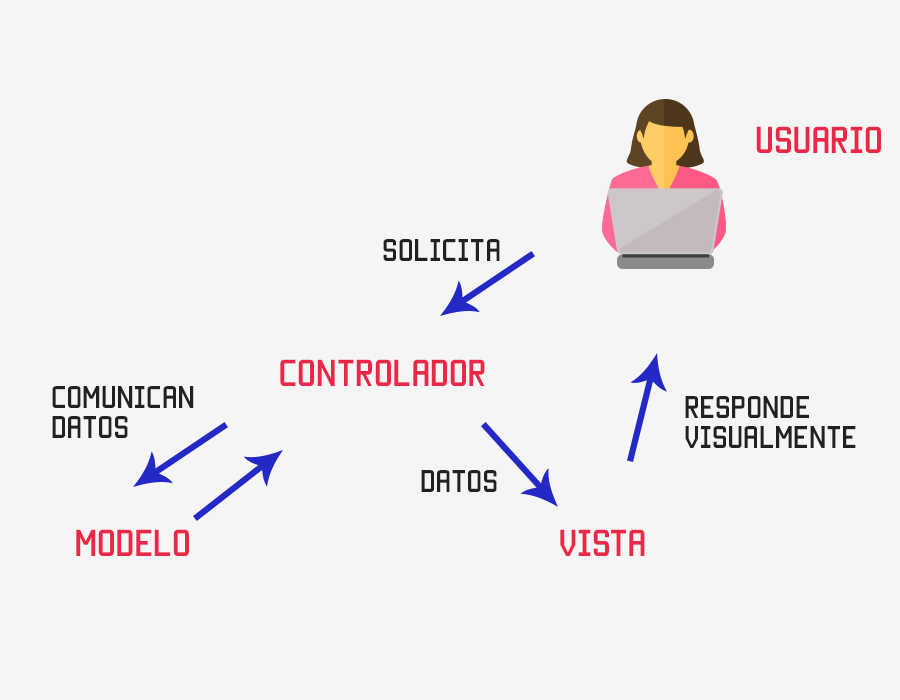
\includegraphics[width=0.8\textwidth]{imagenes/04_Analisis/ciclo_vida_MVC.jpg}
    \begin{center}
        (Fuente: \url{https://codigofacilito.com/articulos/mvc-model-view-controller-explicado})
    \end{center}
    \caption{Ciclo de vida de MVC}
\end{figure}

\subsection{Adaptación del proyecto a la arquitectura}




\chapter{Diseño}




\chapter{Implementación}





\chapter{Pruebas}





\chapter{Conclusiones y posibles ampliaciones}





\nocite{*}
\bibliographystyle{plain}
\bibliography{bibliografia/bibliografia}\addcontentsline{toc}{chapter}{Bibliografía}

%
%%\chapter{Conclusiones y Trabajos Futuros}
%
%


%
%\appendix
%\chapter{Manual de usuario}
%%\input{apendices/paper/paper}
%
\makeglossaries


\newglossaryentry{world_wide_web}
{
    name=World Wide Web,
    description={La World Wide Web (W3) fue desarrollada por un conjunto de personas, de entre las que destaca Tim Berners-Lee, a finales de la década de los ochenta. El motivo por el que surgió este desarrollo fue el interés por parte del CERN de poder compartir sus investigaciones con el resto del mundo y por tanto mejorar la comunicación en el mundo investigador.}
}

\newglossaryentry{bot}
{
    name=bot,
    description={Un bot \footnote{https://dictionary.cambridge.org/es-LA/dictionary/english/bot} es un programa informático que trabaja de forma autónoma.}
}

\newglossaryentry{chatbot}
{
    name=chatbot,
    description={Un chatbot \footnote{https://dictionary.cambridge.org/es-LA/dictionary/english/chatbot} es un programa informático diseñado para tener una conversación con un humano, especialmente a través de Internet.}
}

\newglossaryentry{front-end}
{
    name=front-end,
    description={El front-end es la capa que se encuentra por encima del \gls{back-end}. Es la capa visible para el usuario y también es con la que interactúa. Debido a se interactúa con ella debe cumplir unos estándares de usabilidad y estética. Los principales lenguajes de programación con los que se implementa esta capa son: Javascript, CSS y HTML.}
}

\newglossaryentry{back-end}
{
    name=back-end,
    description={El back-end es la capa que se encuentra por debajo del \gls{front-end}. Es la capa no visible para el usuario. En ella se encuentra el funcionamiento de la aplicación, incluyendo servidores y bases de datos. No existe un lenguaje de programación específico para esta capa.}
}

\newglossaryentry{full_stack}
{
    name=Full Stack,
    description={La programación Full Stack abarca tanto la programación del \gls{front-end} como la del \gls{back-end}. Los profesionales de esta programación se denominan programadores Full Stack y tienen las habilidades necesarias para administrar un proyecto completo.}
}

\newglossaryentry{responsive}
{
    name=responsive,
    description={Según Brett S. Gardner \cite{RefWorks:RefID:34-2011responsive}, el diseño responsive de las páginas web permite crear una única página web que es capaz de adaptarse a la interfaz y al contenido de la misma para poder ser visible en distintos dispositivos (móviles, tablets y ordenadores). Este diseño permite mejorar la experiencia del usuario. Actualmente el diseño responsive se implementa a través del lenguaje CSS, en concreto con su versión CSS3, la cuál tiene un enfoque centrado en el usuario permitiendo el diseño de aplicaciones web dinámicas.}
}

\newglossaryentry{API REST}
{
    name=API REST,
    description={Una API REST es un \gls{API} que sigue los principios de diseño de REST. El principal objetivo de estos principios es tener una \gls{API} que posibilite la separación entre cliente y servidor, para ello algunos de sus principios son por ejemplo: tener un interfaz uniforme, es decir, todas las solicitudes hacia un recurso de la API son siempre iguales; o no tener estado, es decir, la API no guarda información, todas la información necesaria para resolver la solicitud debe estar contenida en la misma.}
}

\newglossaryentry{API}
{
    name=API,
    description={Según la página web de IBM \cite{RefWorks:RefID:33-2021-API}, una API o interfaz de programación de aplicaciones, es un conjunto de reglas que determinan cómo las aplicaciones o los dispositivos pueden conectarse y comunicarse entre sí.}
}

\newglossaryentry{Siracusa}
{
    name=Siracusa,
    description={Siracusa es una ciudad de Italia, situada en la costa sudeste de la isla de Sicilia, famosa como centro cultural desde la Antigua Grecia.}
}

\newglossaryentry{Github}
{
    name=Github,
    description={Github es una plataforma donde multitud de personas y empresas desarrollan software. Esta plataforma permite la comunicación e interacción de la comunidad de desarrolladores de software. Los proyectos se alojan en lo que se denominan repositorios, los cuáles pueden ser públicos o privados. Cada repositorio tiene un control de versiones mediante Git.}
}



% \addcontentsline{toc}{chapter}{Glosario}
% \printglossary
\chapter*{}
\thispagestyle{empty}

\end{document}
